\documentclass[compress]{beamer}
\usepackage{ifthen,verbatim}

\newcommand{\isnote}{}
\xdefinecolor{lightyellow}{rgb}{1.,1.,0.25}
\xdefinecolor{darkblue}{rgb}{0.1,0.1,0.7}

%% Uncomment this to get annotations
%% \def\notes{\addtocounter{page}{-1}
%%            \renewcommand{\isnote}{*}
%% 	   \beamertemplateshadingbackground{lightyellow}{white}
%%            \begin{frame}
%%            \frametitle{Notes for the previous page (page \insertpagenumber)}
%%            \itemize}
%% \def\endnotes{\enditemize
%% 	      \end{frame}
%%               \beamertemplateshadingbackground{white}{white}
%%               \renewcommand{\isnote}{}}

%% Uncomment this to not get annotations
\def\notes{\comment}
\def\endnotes{\endcomment}

\setbeamertemplate{navigation symbols}{}
\setbeamertemplate{headline}{\mbox{ } \hfill
\begin{minipage}{5.5 cm}
\vspace{-0.75 cm} \small
\end{minipage} \hfill
\begin{minipage}{4.5 cm}
\vspace{-0.75 cm} \small
\begin{flushright}
\ifthenelse{\equal{\insertpagenumber}{1}}{}{Jim Pivarski \hspace{0.2 cm} \insertpagenumber\isnote/\pageref{numpages}}
\end{flushright}
\end{minipage}\mbox{\hspace{0.2 cm}}\includegraphics[height=1 cm]{../cmslogo} \hspace{0.1 cm} \includegraphics[height=1 cm]{../tamulogo} \hspace{0.01 cm} \vspace{-1.05 cm}}

\begin{document}
\begin{frame}
\vfill
\begin{center}
\textcolor{darkblue}{\Large HW-track Comparison and Tracker Global Shape}

\vfill
\begin{columns}
\column{0.3\linewidth}
\begin{center}
\large
\textcolor{darkblue}{Jim Pivarski}
\end{center}
\end{columns}

\begin{columns}
\column{0.3\linewidth}
\begin{center}
\scriptsize
{\it Texas A\&M University}
\end{center}
\end{columns}

\vfill
 4 December, 2009

\end{center}
\end{frame}

%% \begin{notes}
%% \item This is the annotated version of my talk.
%% \item If you want the version that I am presenting, download the one
%% labeled ``slides'' on Indico (or just ignore these yellow pages).
%% \item The annotated version is provided for extra detail and a written
%% record of comments that I intend to make orally.
%% \item Yellow notes refer to the content on the {\it previous} page.
%% \item All other slides are identical for the two versions.
%% \end{notes}

\small

\begin{frame}
\frametitle{Outline}
\begin{itemize}\setlength{\itemsep}{0.75 cm}
\item Hardware alignment as seen by tracks
\item Resolving tracker global distortions with muon residuals
\end{itemize}
%% \hspace{-0.83 cm} \textcolor{darkblue}{\Large Outline2}
\end{frame}

\begin{frame}
\frametitle{New hardware alignment}

\begin{columns}
\column{0.7\linewidth}
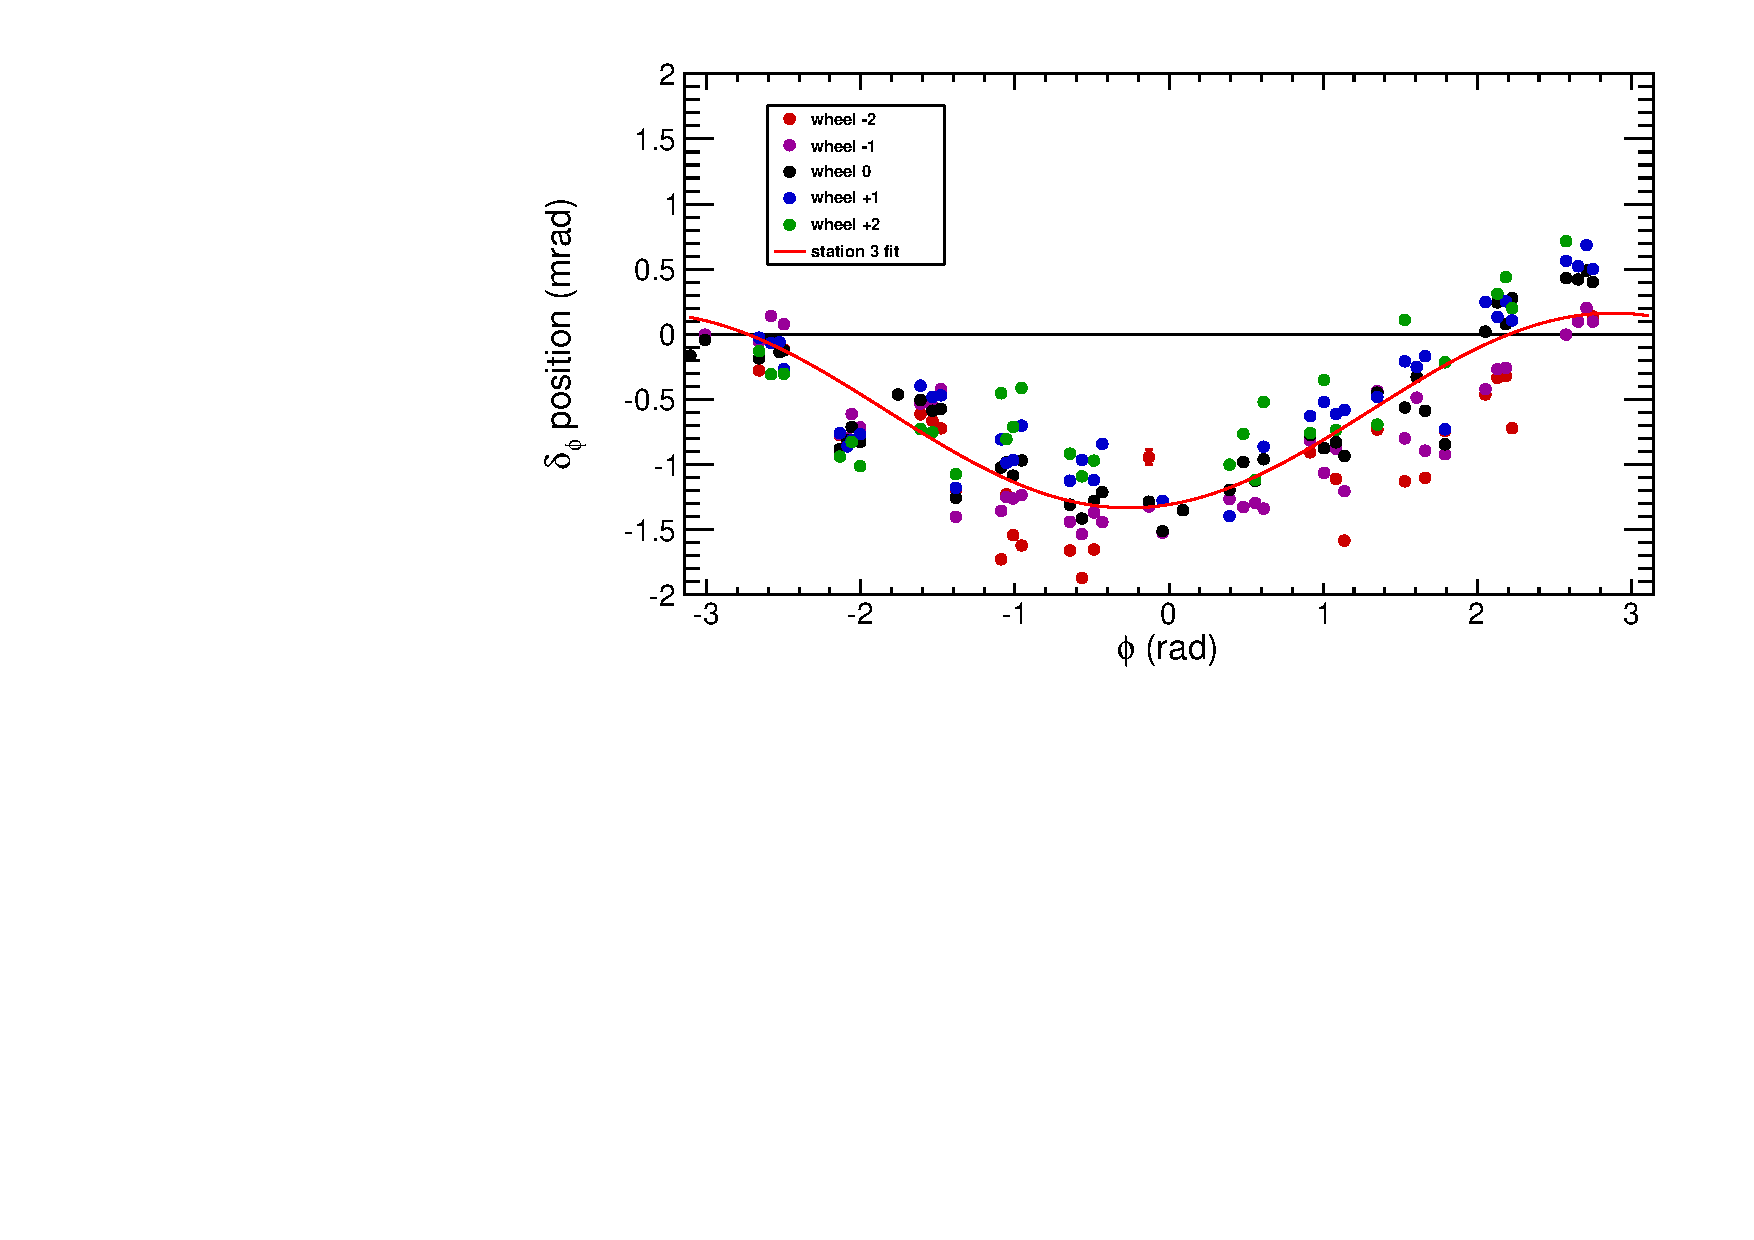
\includegraphics[width=\linewidth]{NovHardware_vs_phi.pdf}

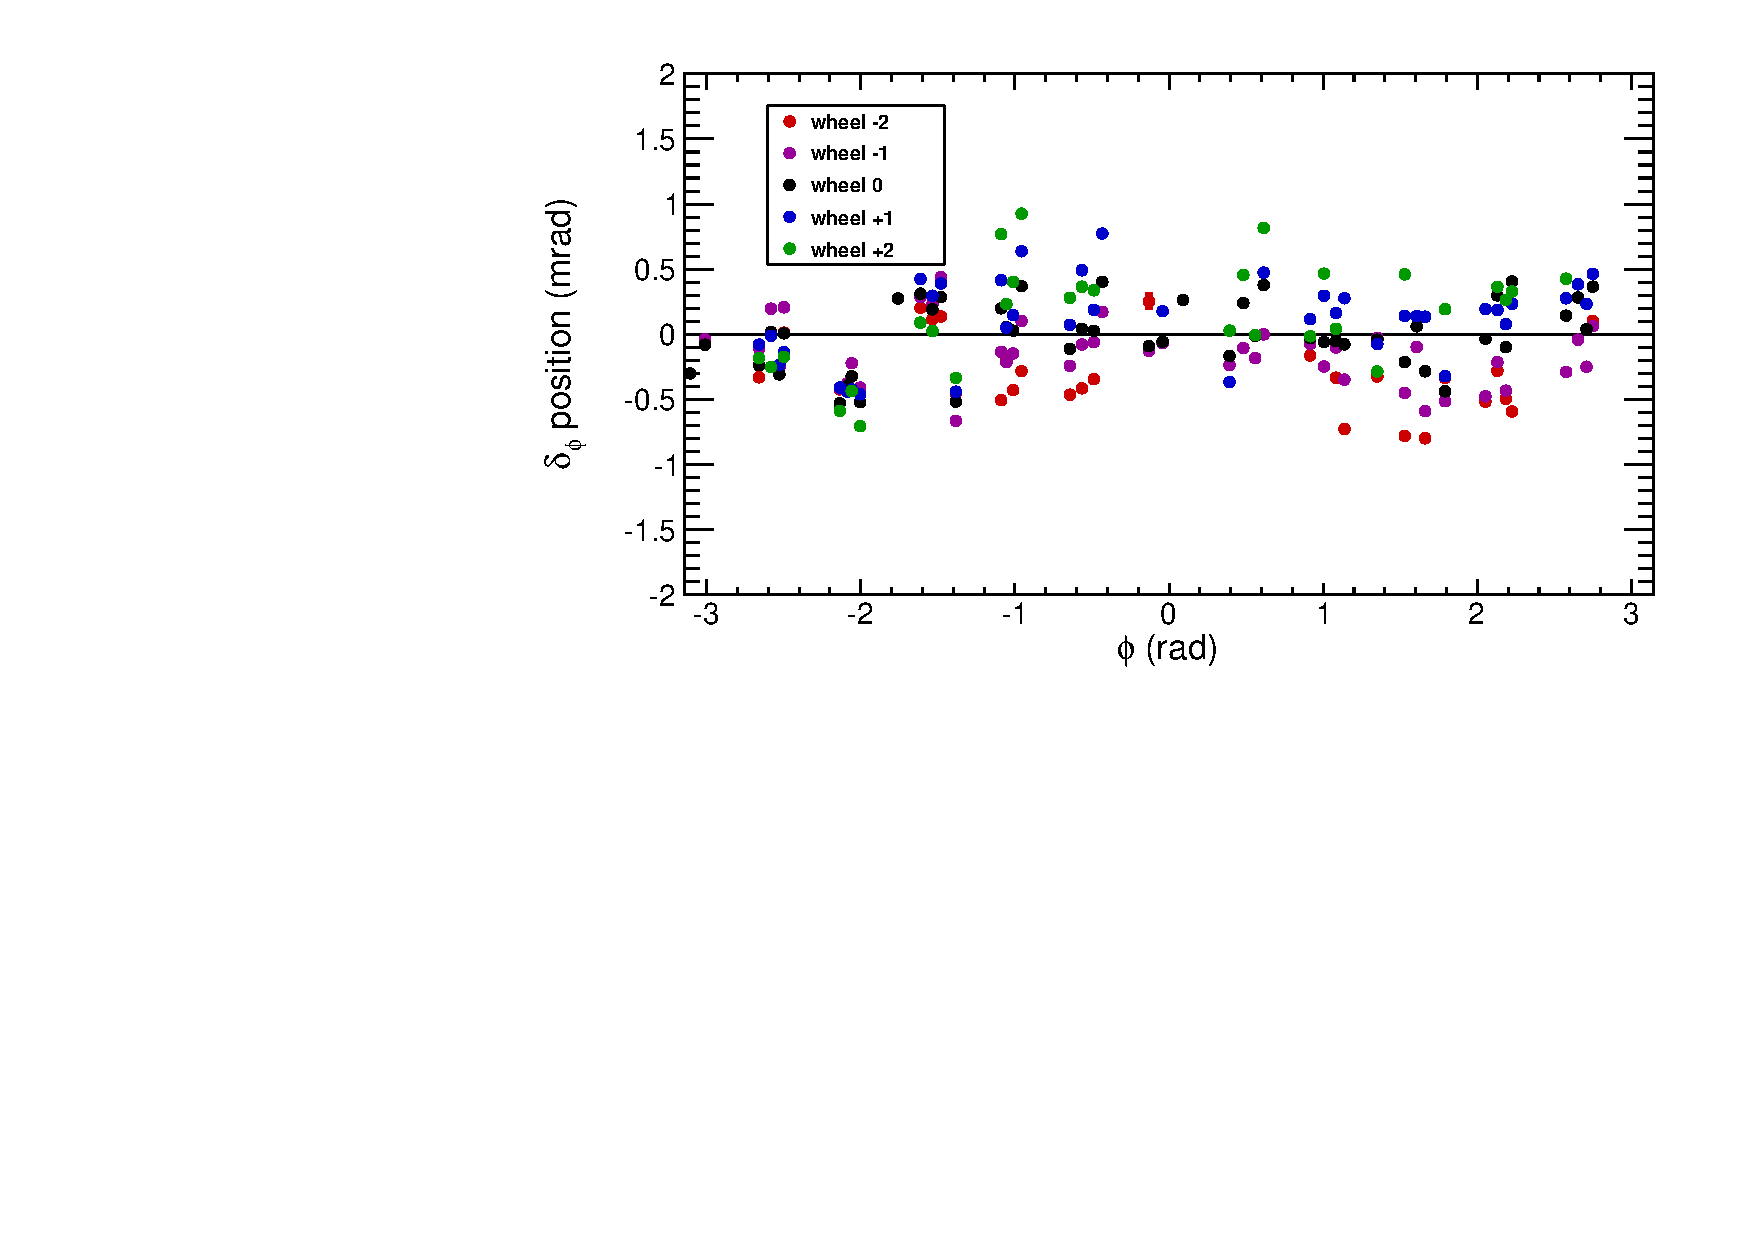
\includegraphics[width=\linewidth]{NovHardwareADJUSTED_vs_phi.pdf}

\column{0.4\linewidth}
\begin{itemize}
\item Nov 19 Link-fixed HW barrel alignment

\item $\phi = x / R$

\item Much more consistent with a single offset of the tracker
\begin{itemize}
\item $x \to 1.2$~mm
\item $y \to 4.5$~mm
\item $\phi_z \to 0.58$~mrad
\end{itemize}

\item See \textcolor{blue}{https://hypernews. cern.ch/HyperNews/ CMS/get/muon-alignment/423/1.html} or Nov 20 Indico page for the full set of plots

\end{itemize}
\end{columns}
\end{frame}

\begin{frame}
\frametitle{After global adjustment}

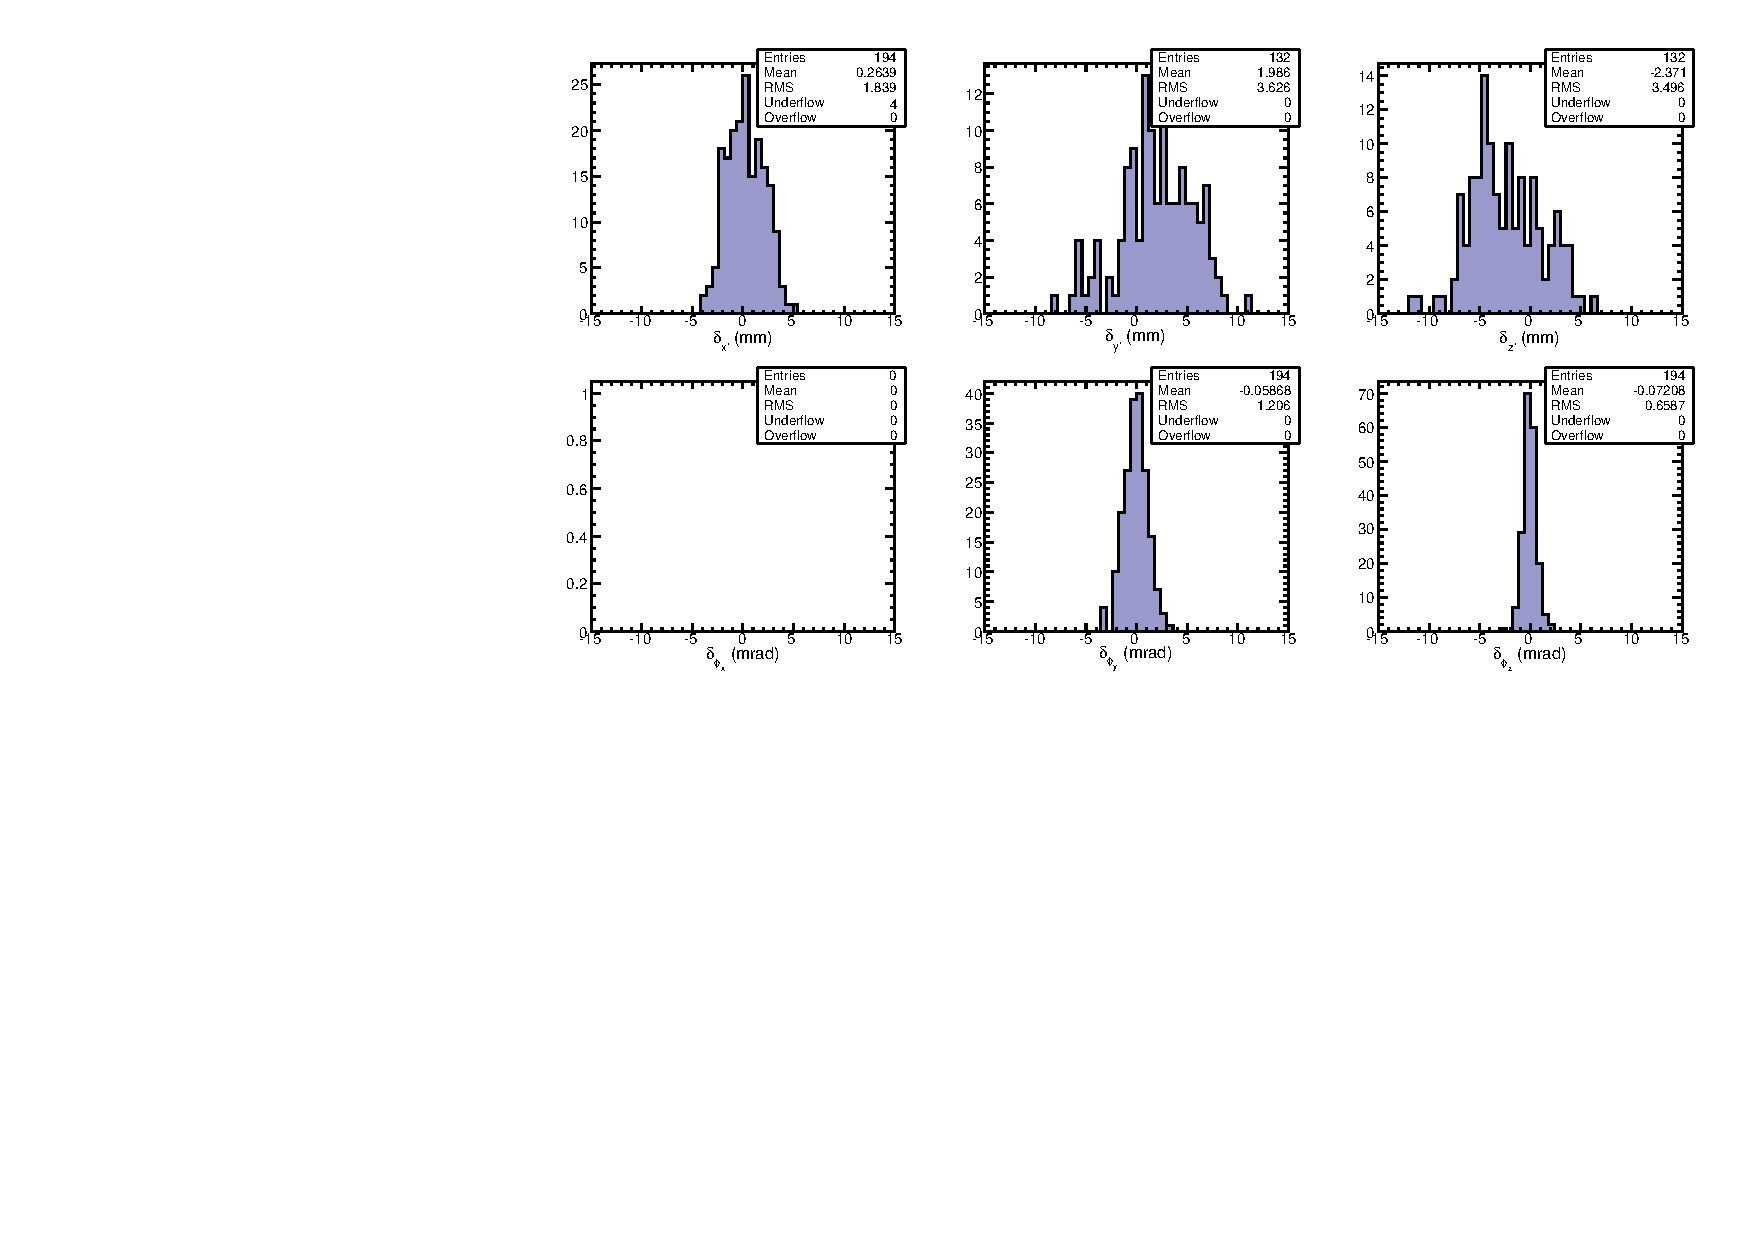
\includegraphics[width=\linewidth]{NovHardware_vs_tracks_as_histograms.pdf}

\begin{itemize}
\item RMS of $x'$ deviations (top-left) is only 1.8~mm after removing global offset in transverse plane

\item Similar to photogrammetry, which had an RMS of 1.6~mm
\end{itemize}
\end{frame}

\begin{frame}
\frametitle{Other translational d.o.f.}

\begin{columns}
\column{0.7\linewidth}
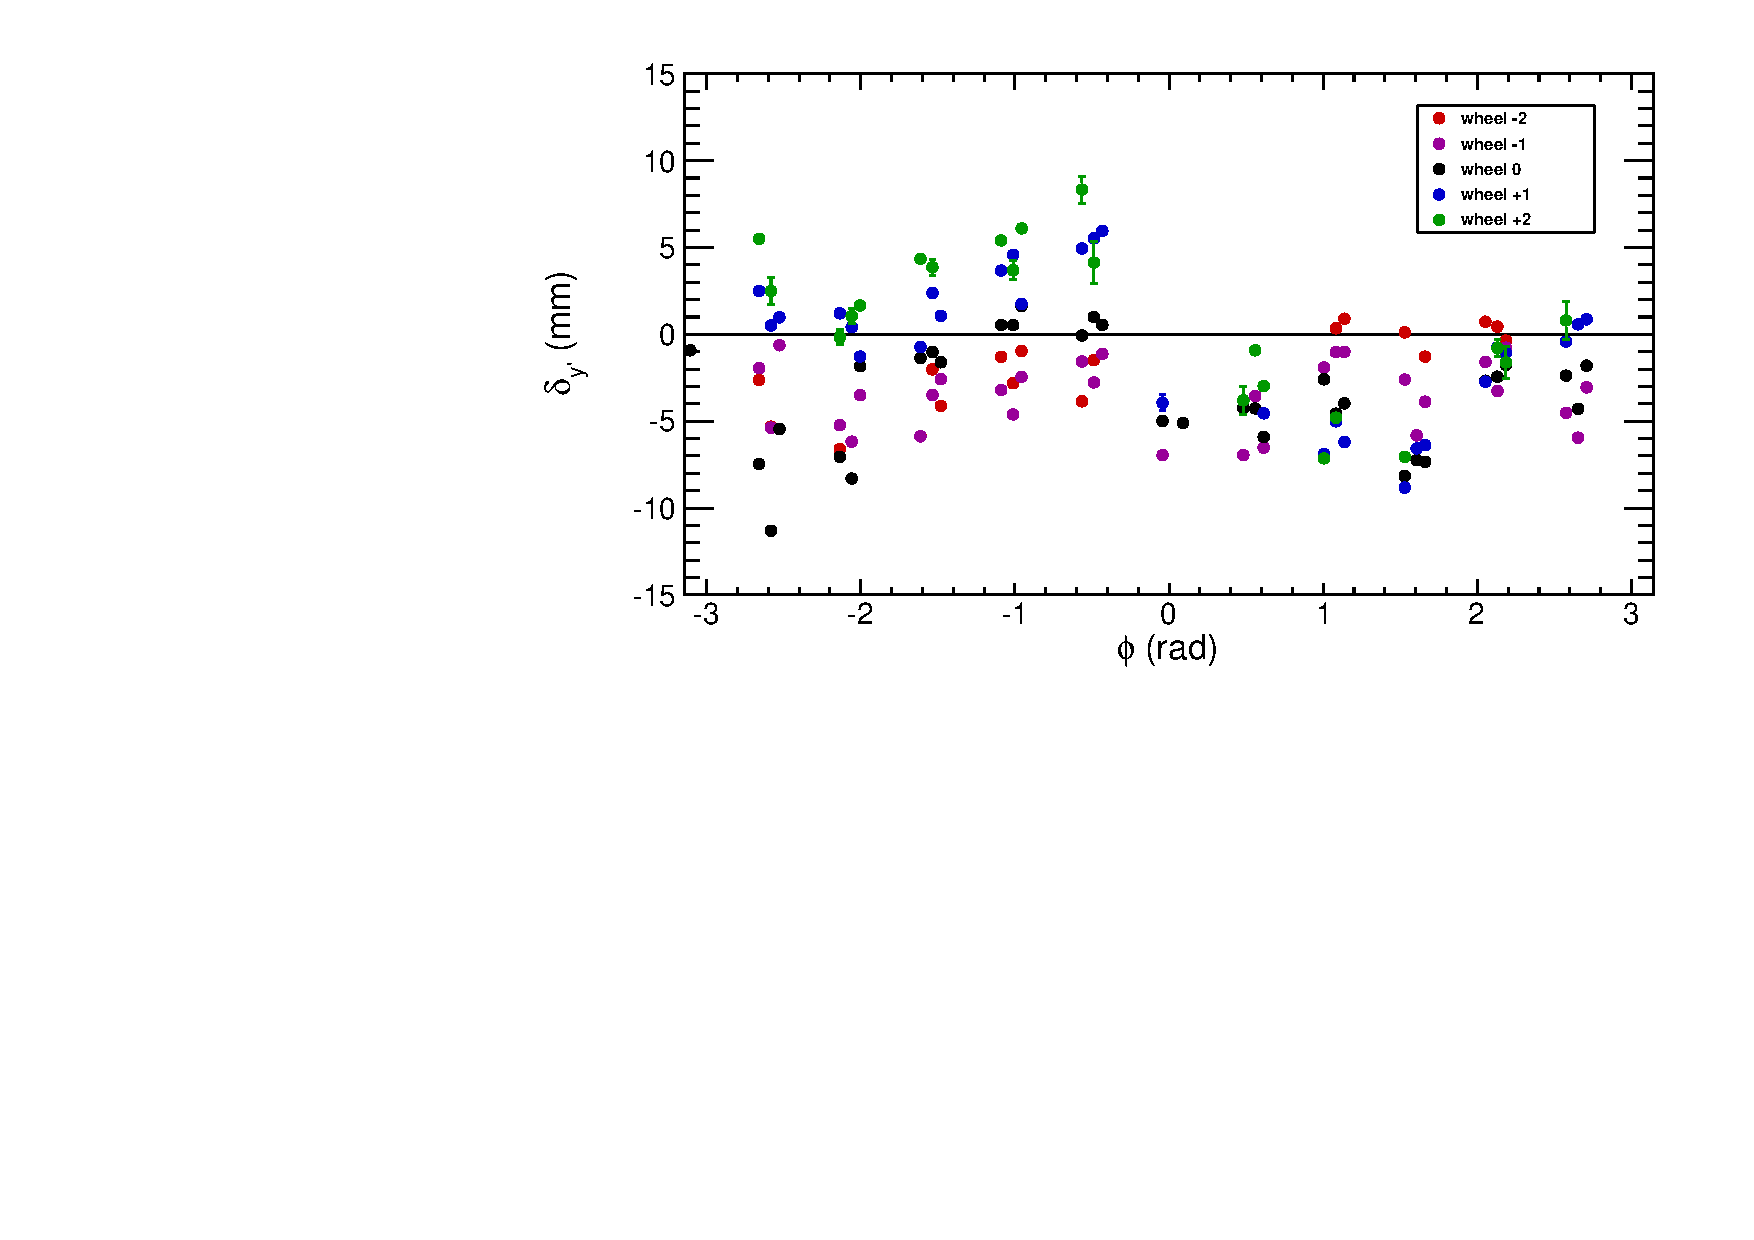
\includegraphics[width=\linewidth]{NovHardwareADJUSTED_vs_y.pdf}

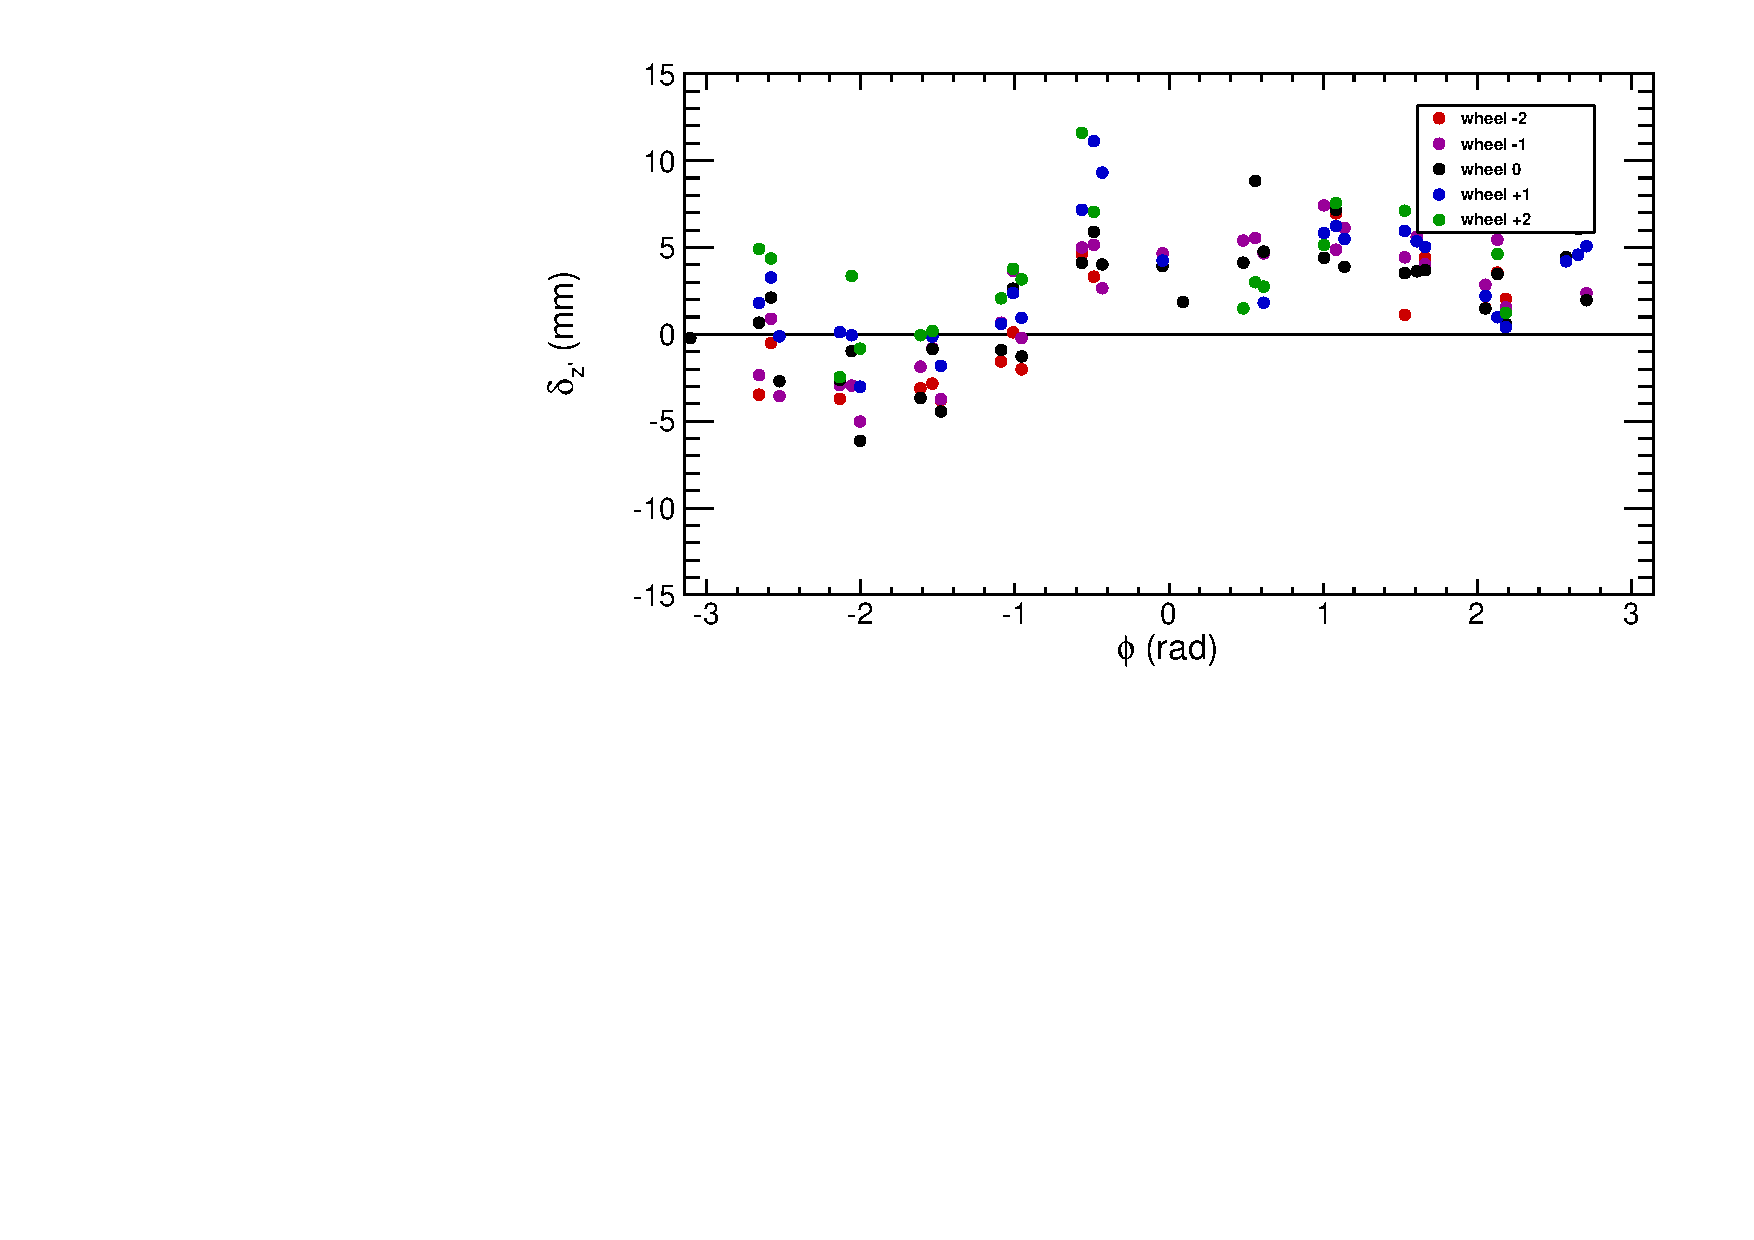
\includegraphics[width=\linewidth]{NovHardwareADJUSTED_vs_z.pdf}

\column{0.4\linewidth}
\begin{itemize}
\item Top: $y'$ differences (direction parallel to beamline)

\item Bottom: $z'$ differences (radial)

\item These are more consistent within sector groups

\item $y'$ has a clear trend with respect to wheel
\end{itemize}
\end{columns}
\end{frame}

\begin{frame}
\frametitle{Map plots}

\begin{center}
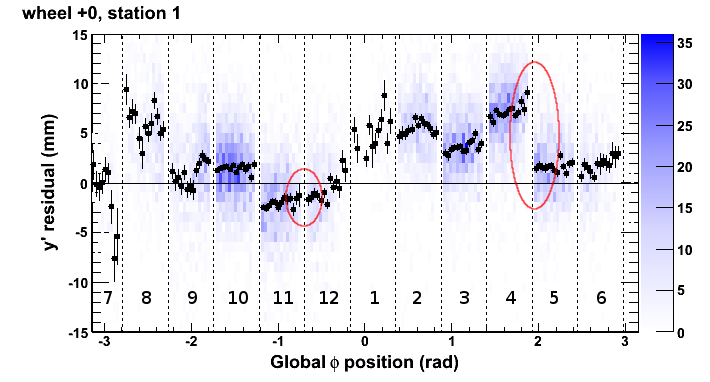
\includegraphics[width=0.8\linewidth]{DTvsphi_st1whC_y.png}
\end{center}

\vspace{-0.5 cm}
\begin{itemize}
\item Map plots show that the remaining differences are not due to tracker distortions
\item For example, the statement ``relative misalignment of sectors 4 and 5 is 6~mm'' is tracker-independent and propagation-independent
\item When the hardware geometry correctly describes the muon system as a rigid body, the differences with respect to track-based will be a {\it smooth} function in these plots (e.g. between sectors 11 and 12)
\end{itemize}
\end{frame}

\begin{frame}
\frametitle{Resolving tracker distortions}

\begin{itemize}
\item We can identify tracker global distortions using muon chamber data
\item Without introducing circularity when we later align the muon system with tracker tracks
\end{itemize}

\vspace{0.1 cm}
\begin{columns}
\column{0.5\linewidth}
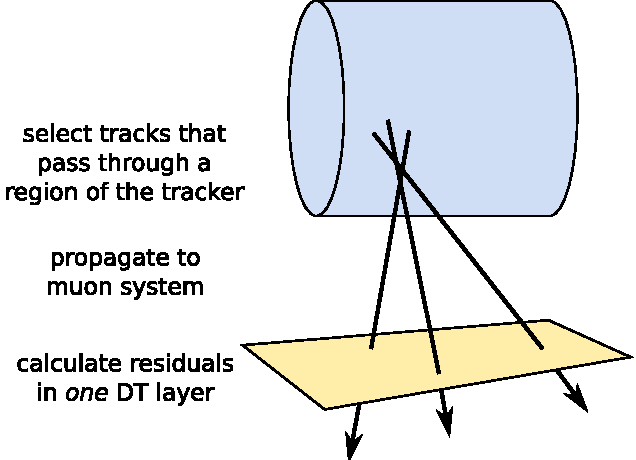
\includegraphics[width=\linewidth]{method.pdf}

\column{0.5\linewidth}
\begin{itemize}
\item Independence from muon alignment: plot residuals in {\it only one muon layer} \\ (wh~0, st~1, sec~10, lay~2) \\ and disregard global position of that layer

\item Look at muon residuals as a function of $p_T$

\item We only assume that the muon layer is in one location that can't be a function of the $p_T$ of the tracks used to measure it
\end{itemize}
\end{columns}

\end{frame}

\begin{frame}
\frametitle{$p_T$-dependent muon residuals}

\begin{columns}
\column{0.57\linewidth}

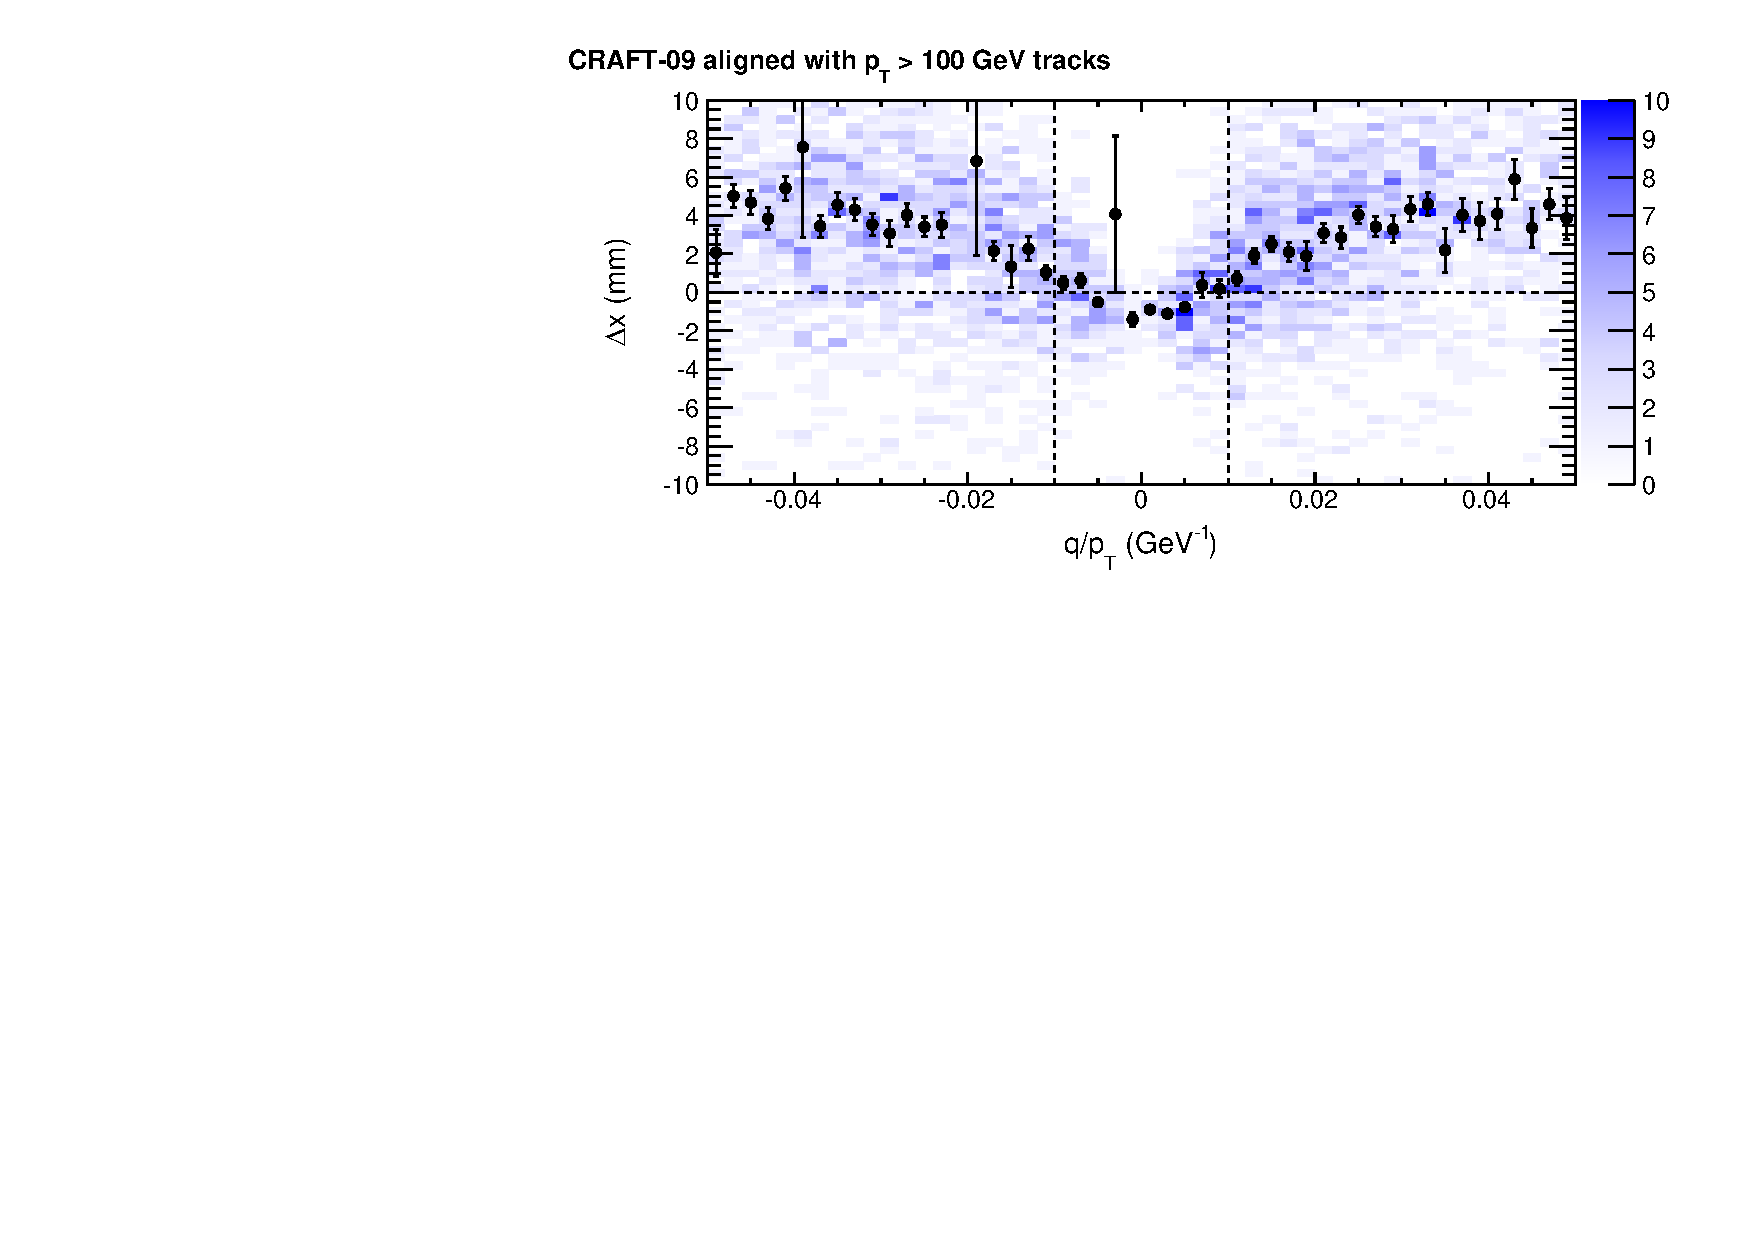
\includegraphics[width=\linewidth]{residuals_real.pdf}

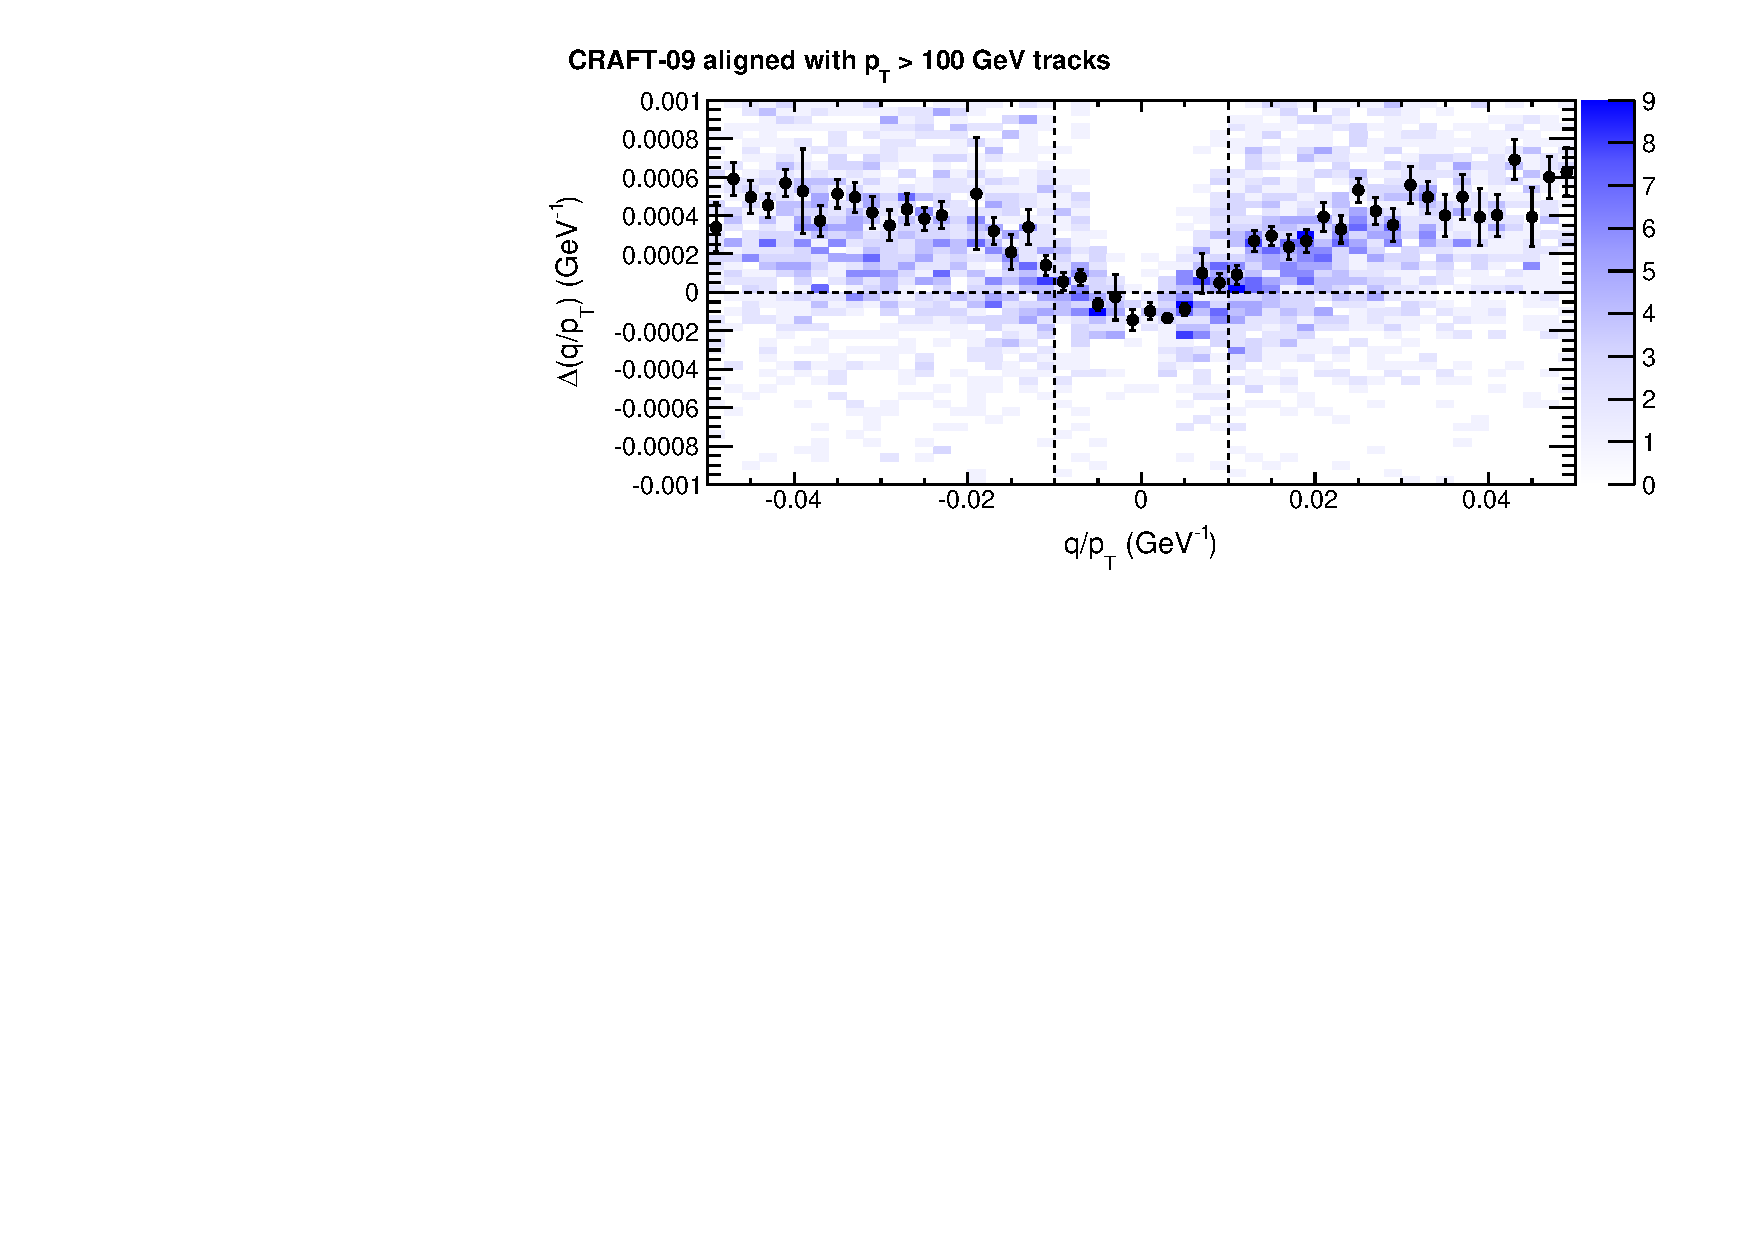
\includegraphics[width=\linewidth]{curvature_real.pdf}

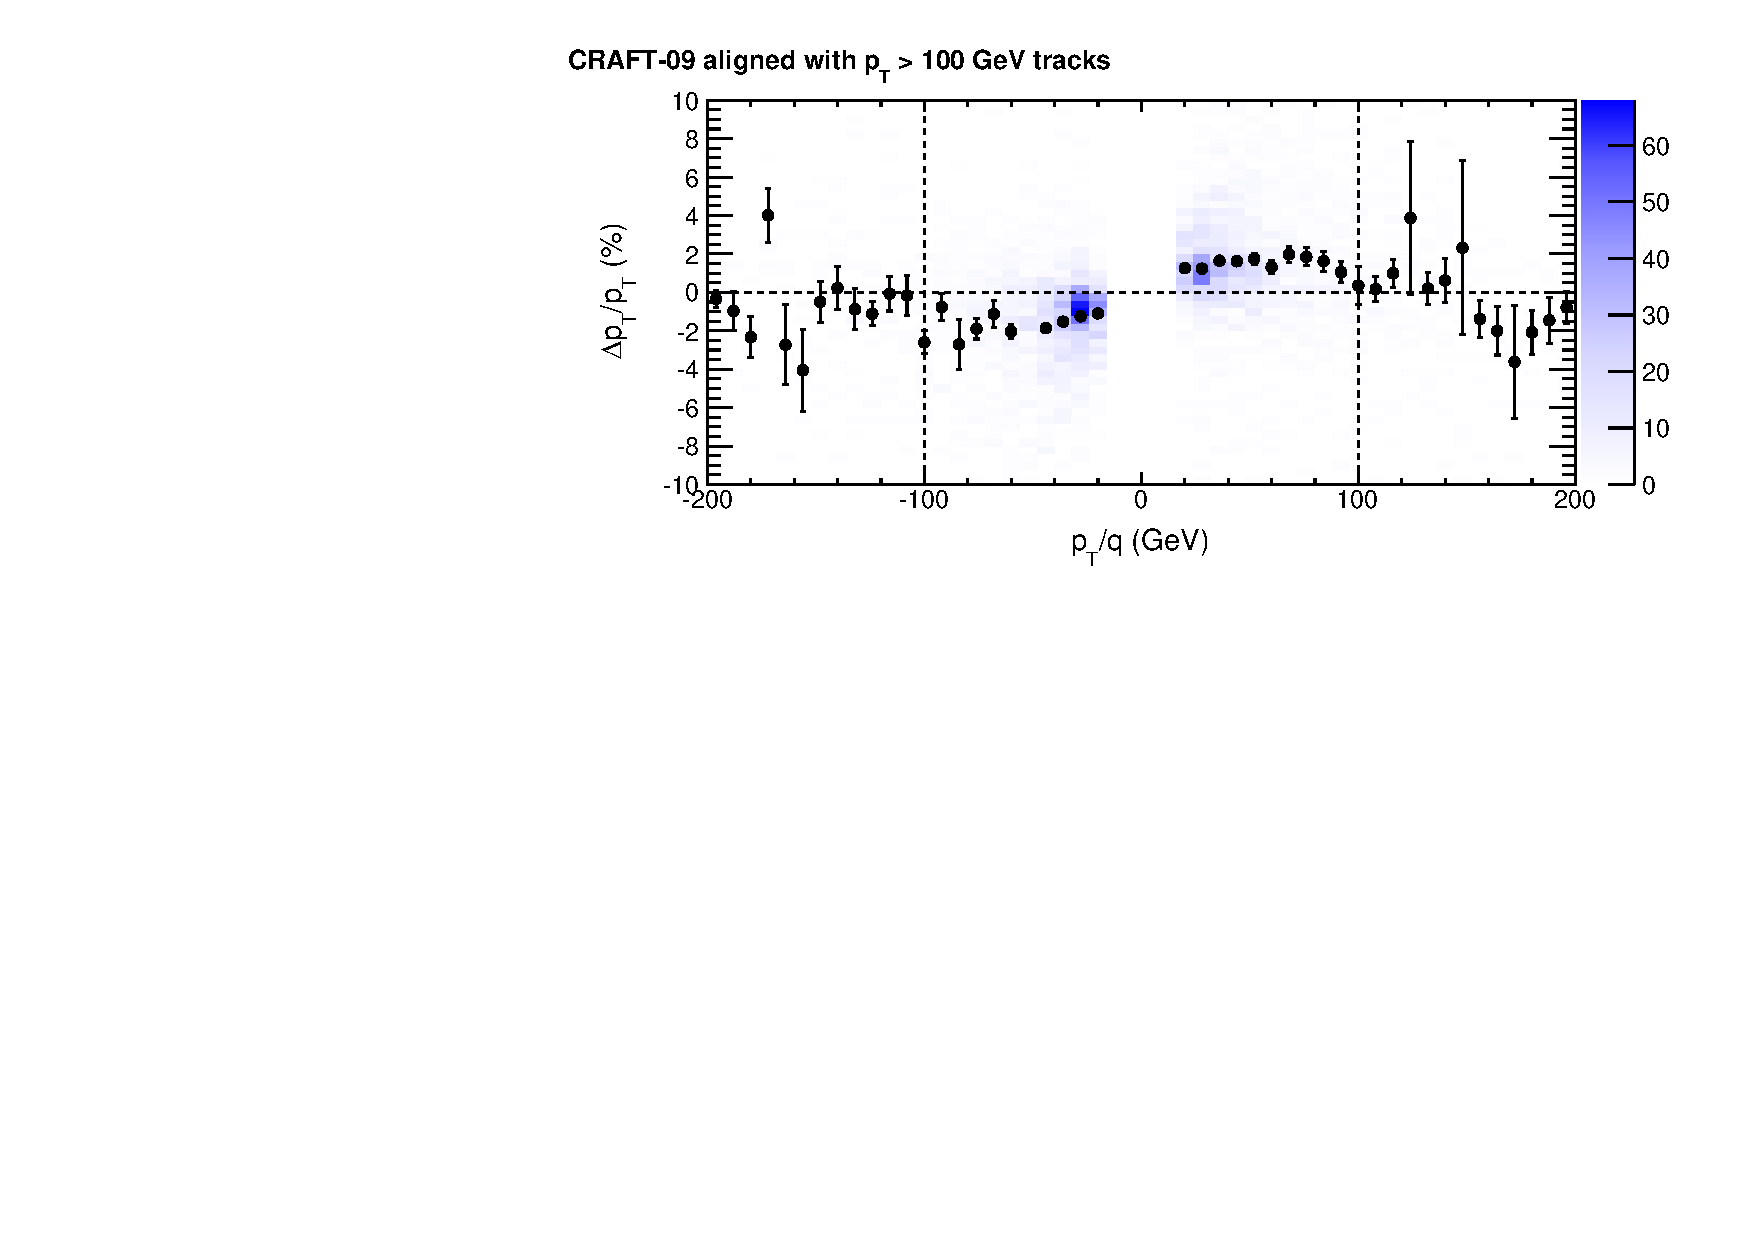
\includegraphics[width=\linewidth]{momenta_real.pdf}

\column{0.5\linewidth}
\begin{itemize}
\item Three ways of looking at it:
\begin{itemize}
\item as a muon residual ($\Delta x$)
\item tracker curvature error ($\Delta \kappa = \Delta x \frac{d\kappa}{dx}$, $\kappa = q/p_T$)
\item tracker momentum error ($\Delta p_T = \Delta x \frac{dp_T}{dx}$)
\end{itemize}
where $\frac{d\kappa}{dx}$ and $\frac{dp_T}{dx}$ come from track propagator, numerically

\item $\frac{d\kappa}{dx}$ is nearly constant for a single DT layer (depends on distance from tracker)

\item From muon hits, we learn something which is purely about the tracker's shape

\item If errors were from $\vec{B}(\vec{x})$ or $dE/dx$, top plot would be antisymmetric, not symmetric
\end{itemize}
\end{columns}
\end{frame}

\begin{frame}
\frametitle{Ambiguity from muon alignment}

\begin{columns}
\column{0.57\linewidth}

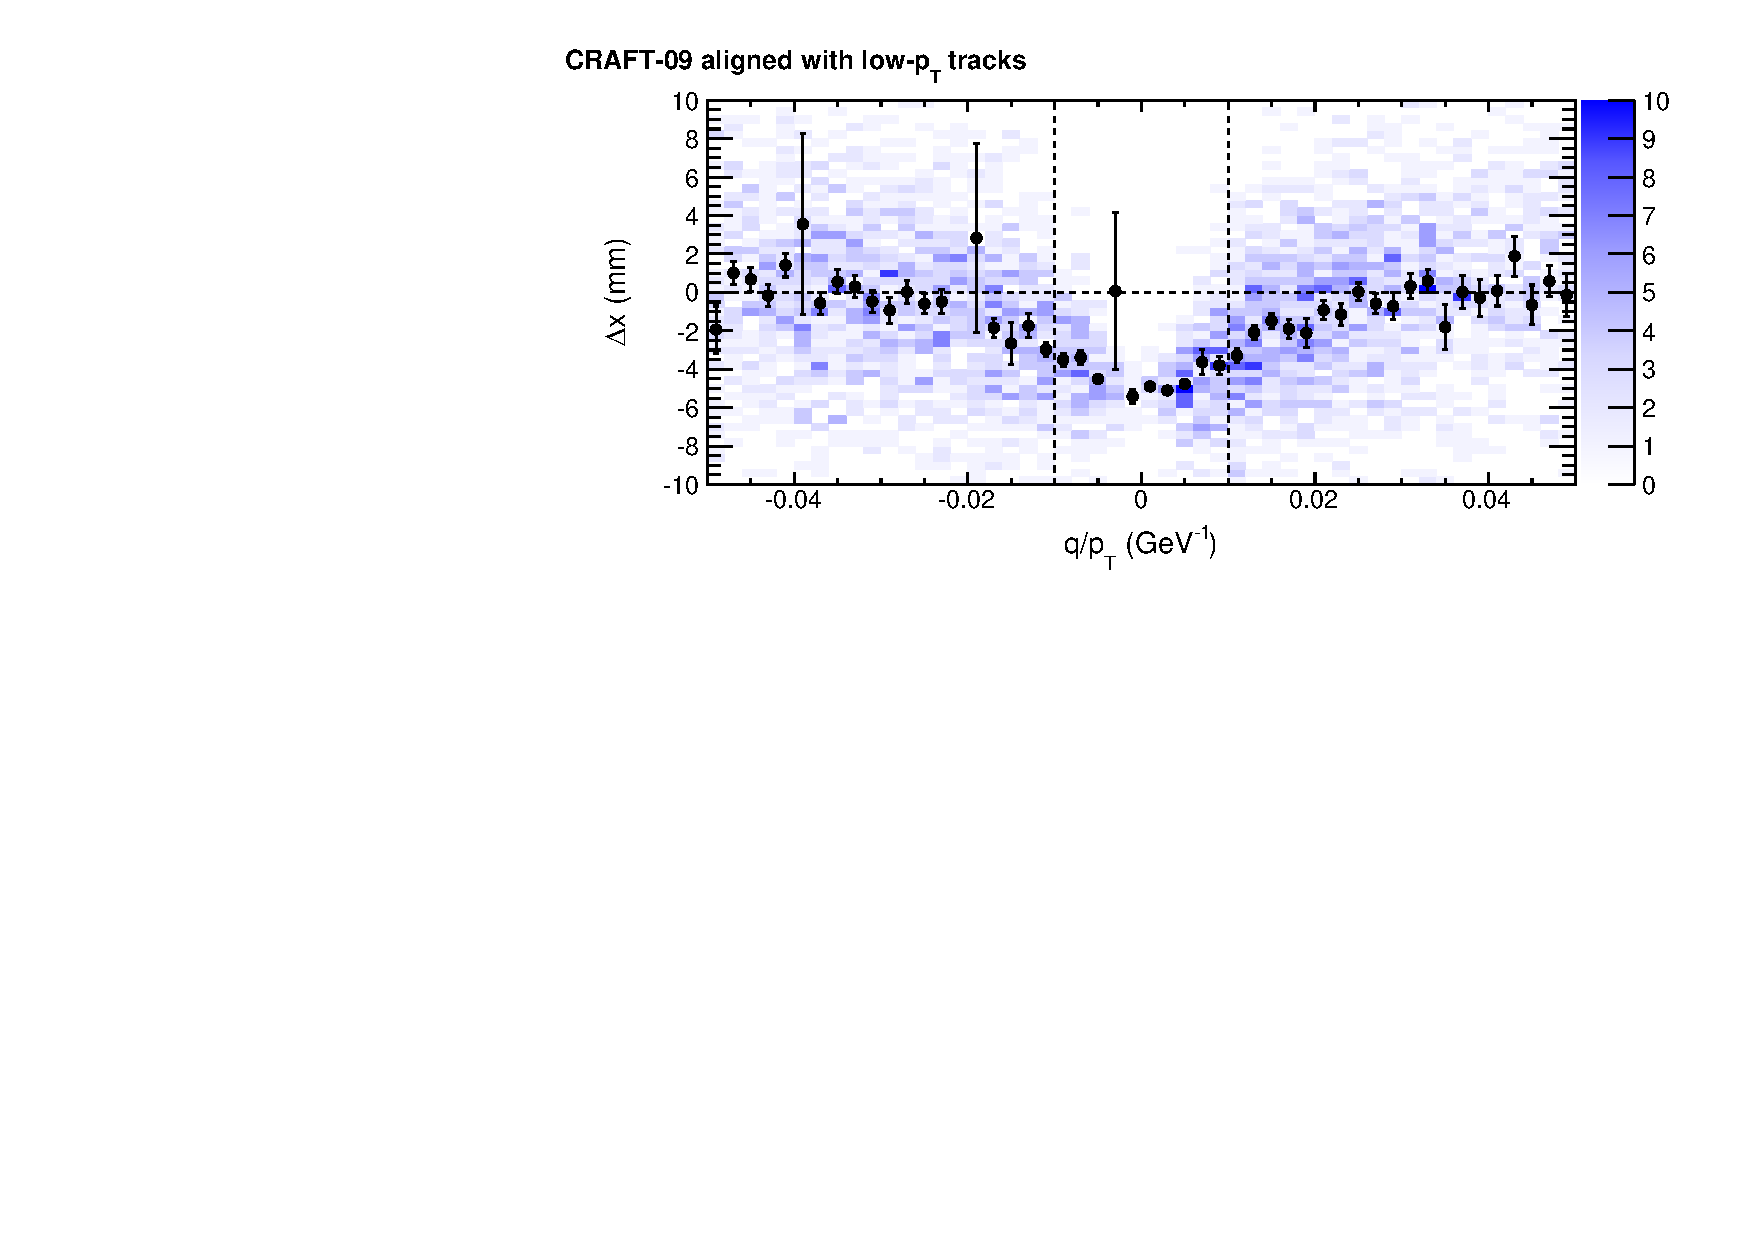
\includegraphics[width=\linewidth]{residuals_realshift.pdf}

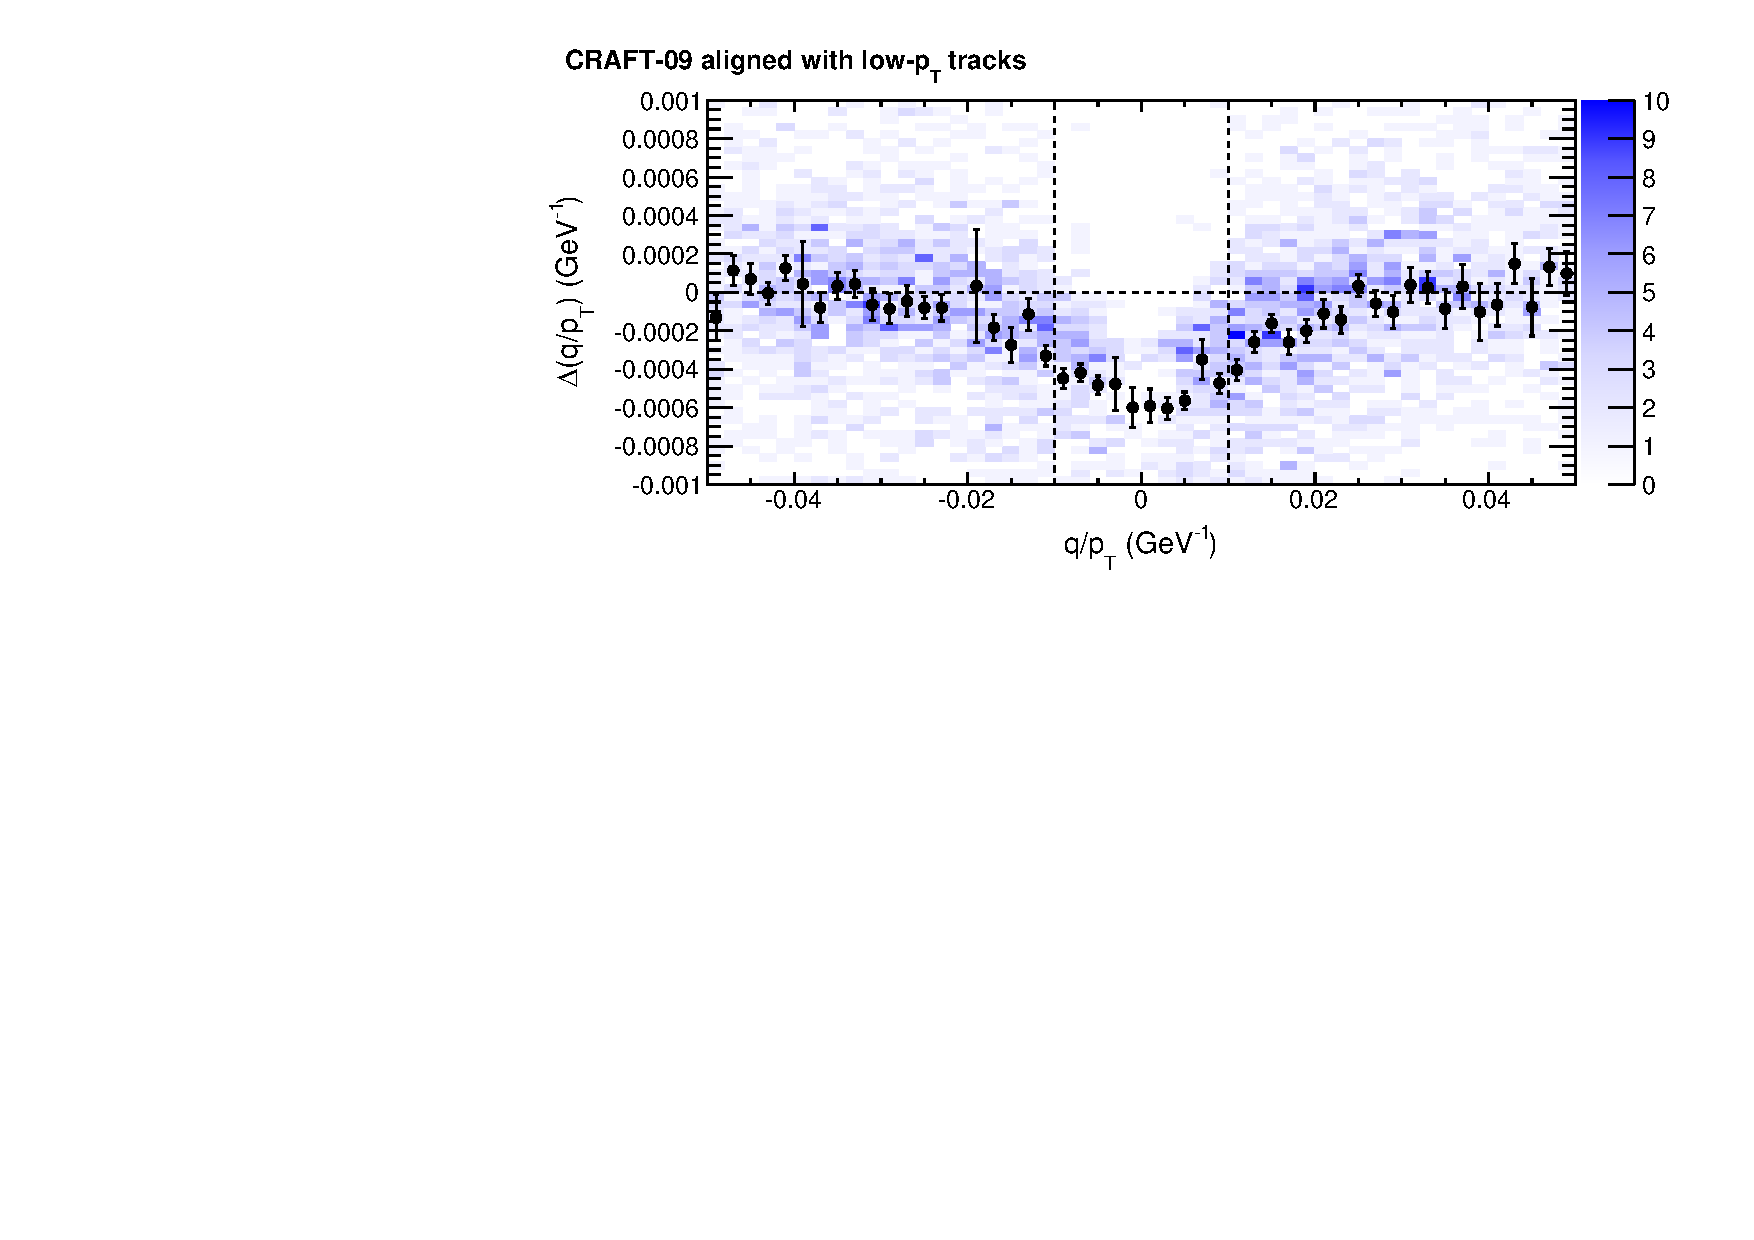
\includegraphics[width=\linewidth]{curvature_realshift.pdf}

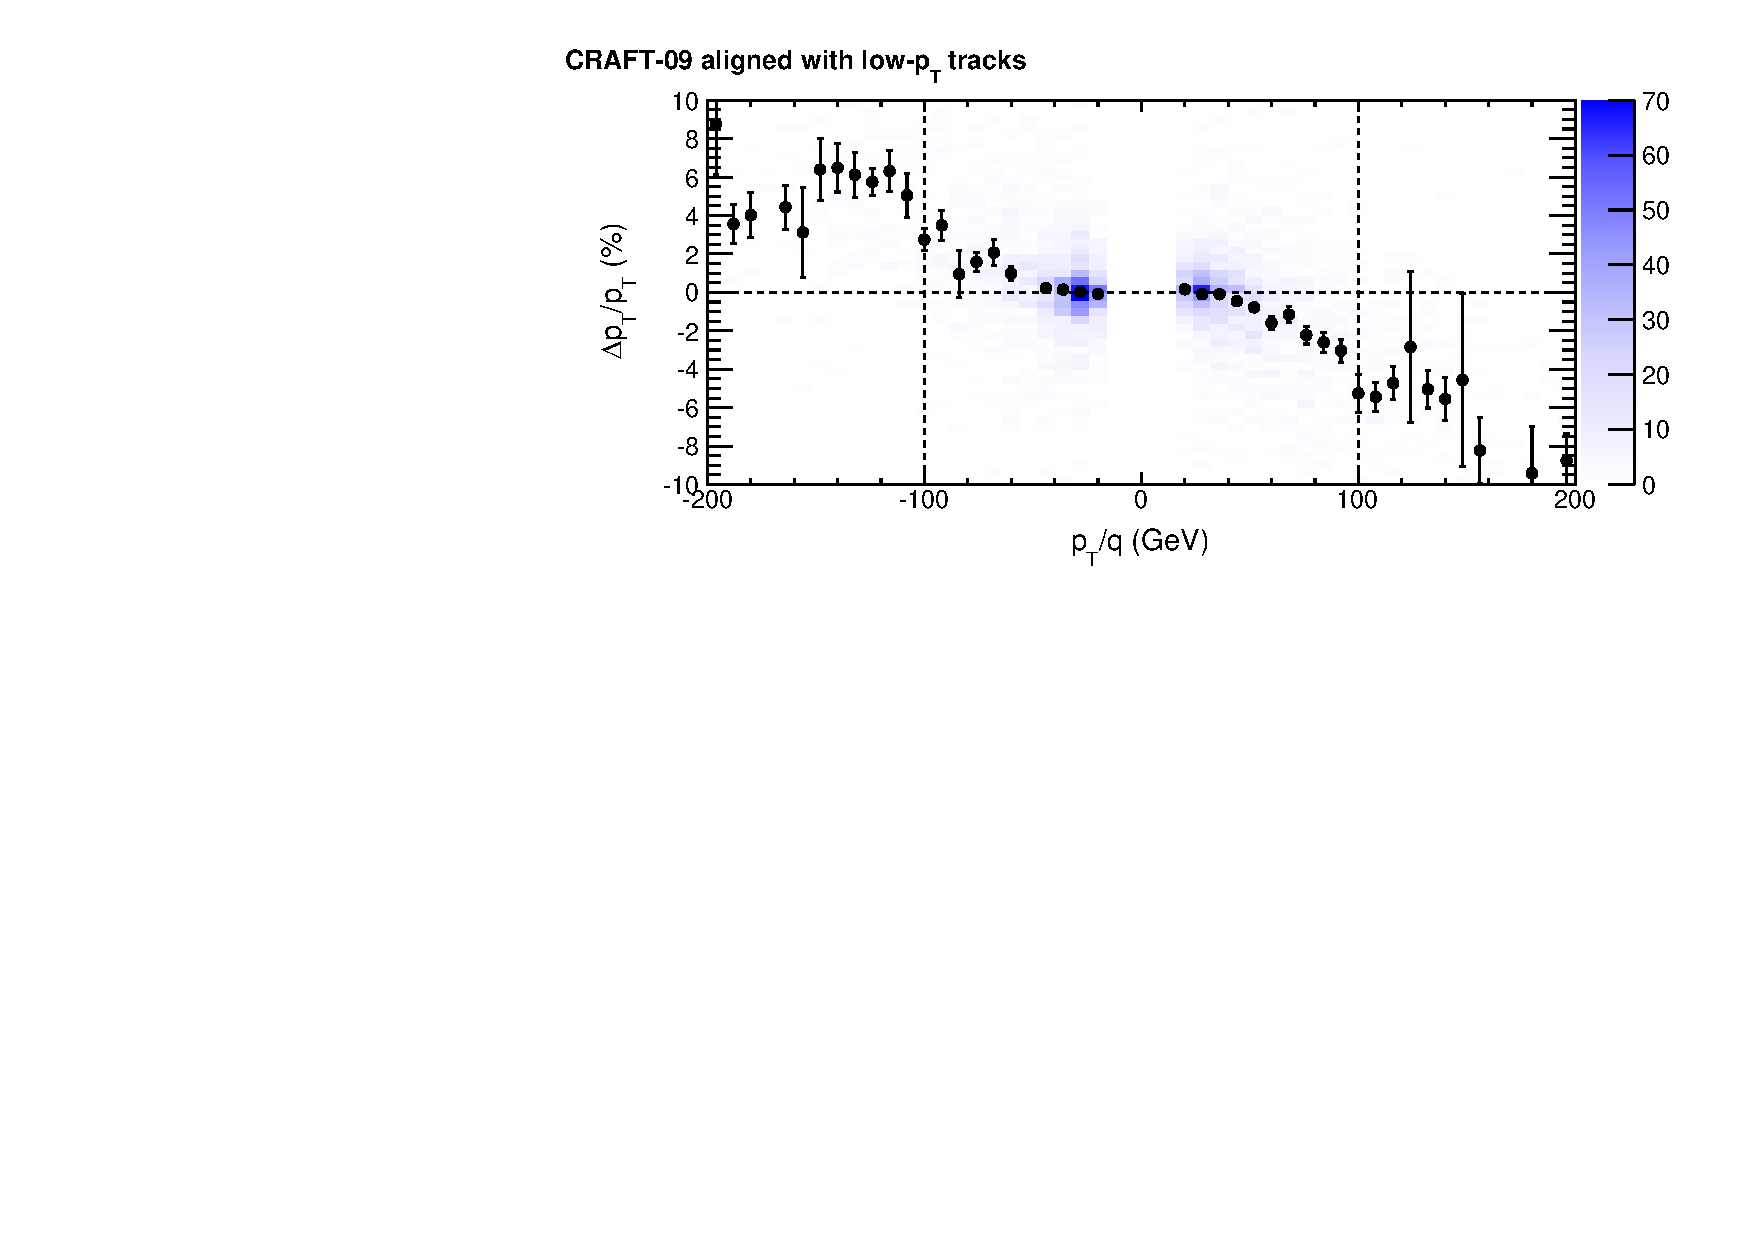
\includegraphics[width=\linewidth]{momenta_realshift.pdf}

\column{0.5\linewidth}
\begin{itemize}
\item To avoid a circular argument, we should keep the position of the muon chamber as a free parameter in this study

\item Knowledge of tracker shape will later be used to determine positions of muon chambers (track-based alignment)

\item Freedom to make low-$p_T$ region ``correct'' and high-$p_T$ region ``wrong''

\item Still, difference in curvature between low- and high-$p_T$ regions is the same: this should constrain models of the tracker's shape
\end{itemize}
\end{columns}
\end{frame}

\begin{frame}
\frametitle{Does this analysis make sense?}

\begin{columns}
\column{0.57\linewidth}

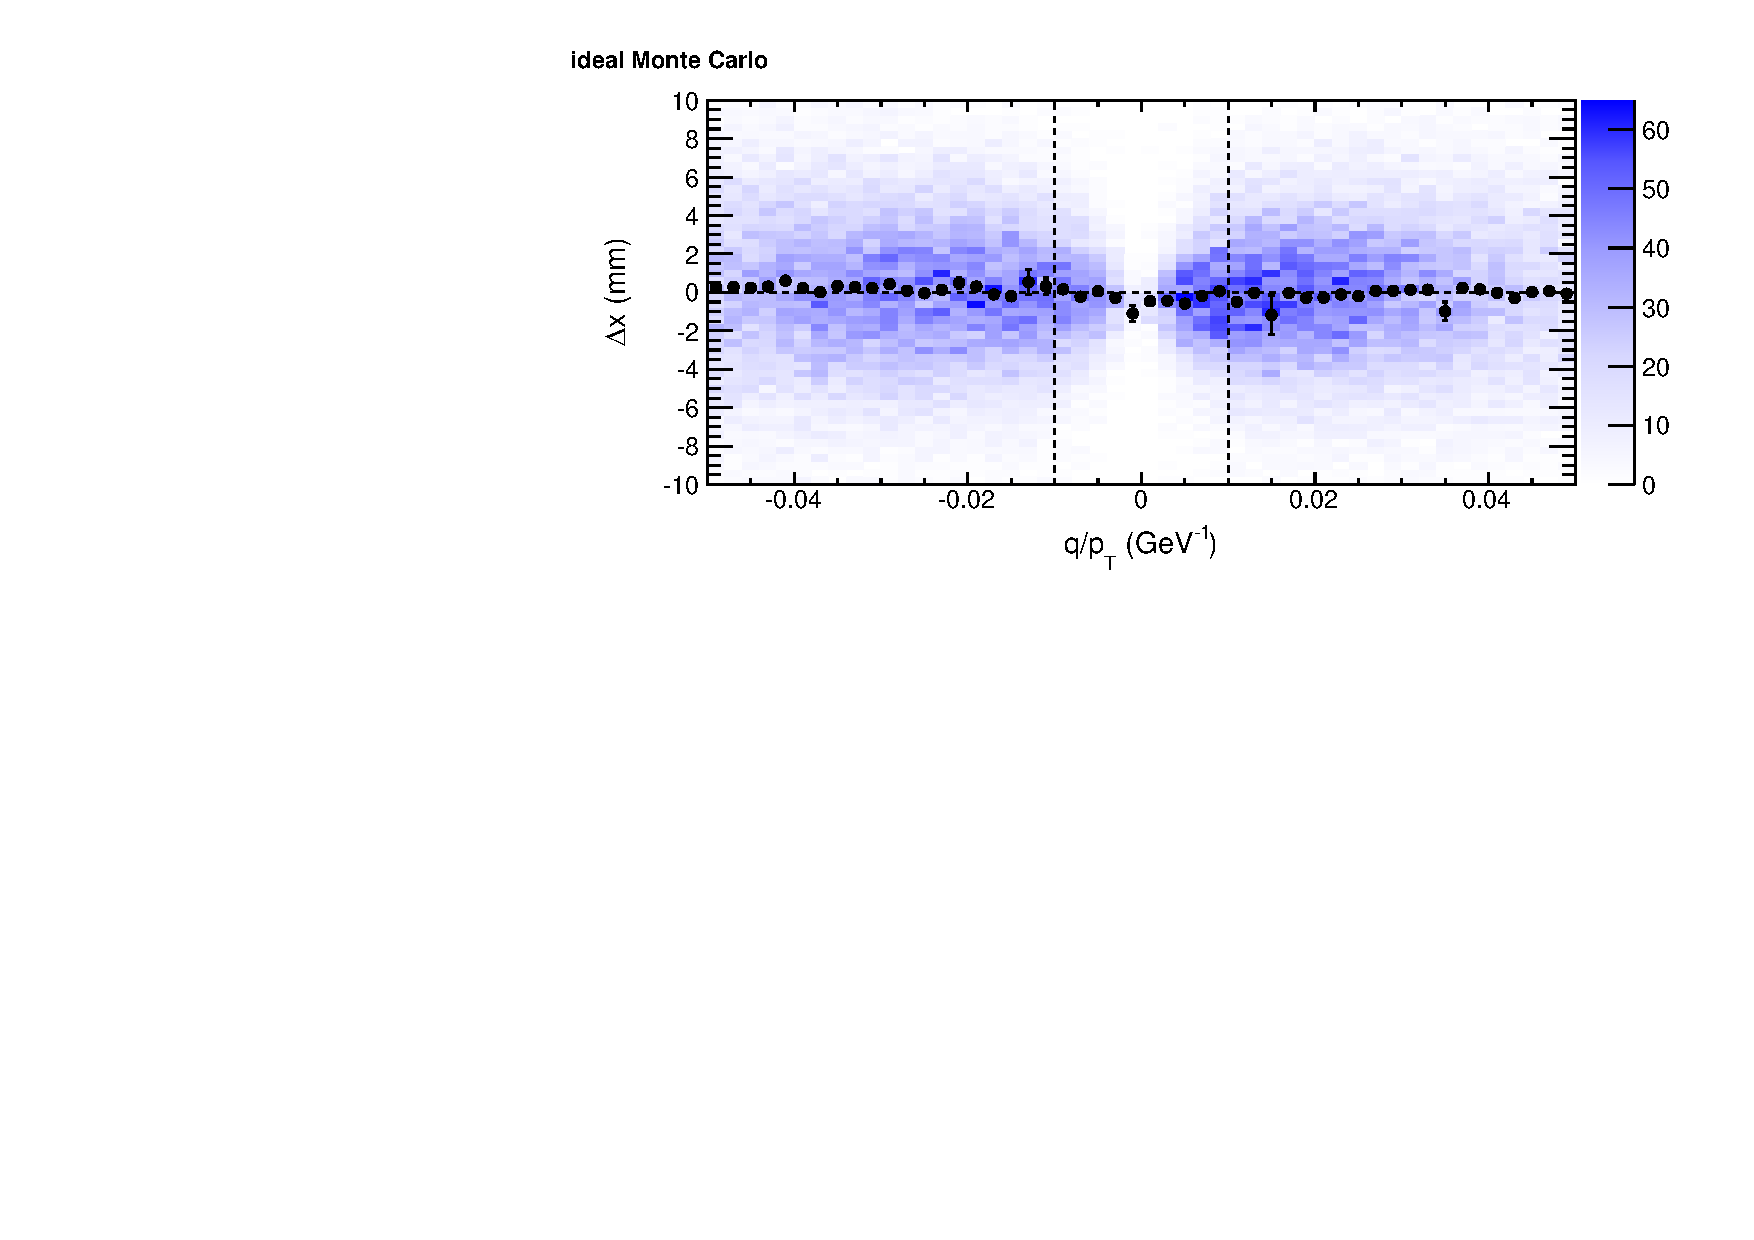
\includegraphics[width=\linewidth]{residuals_ideal.pdf}

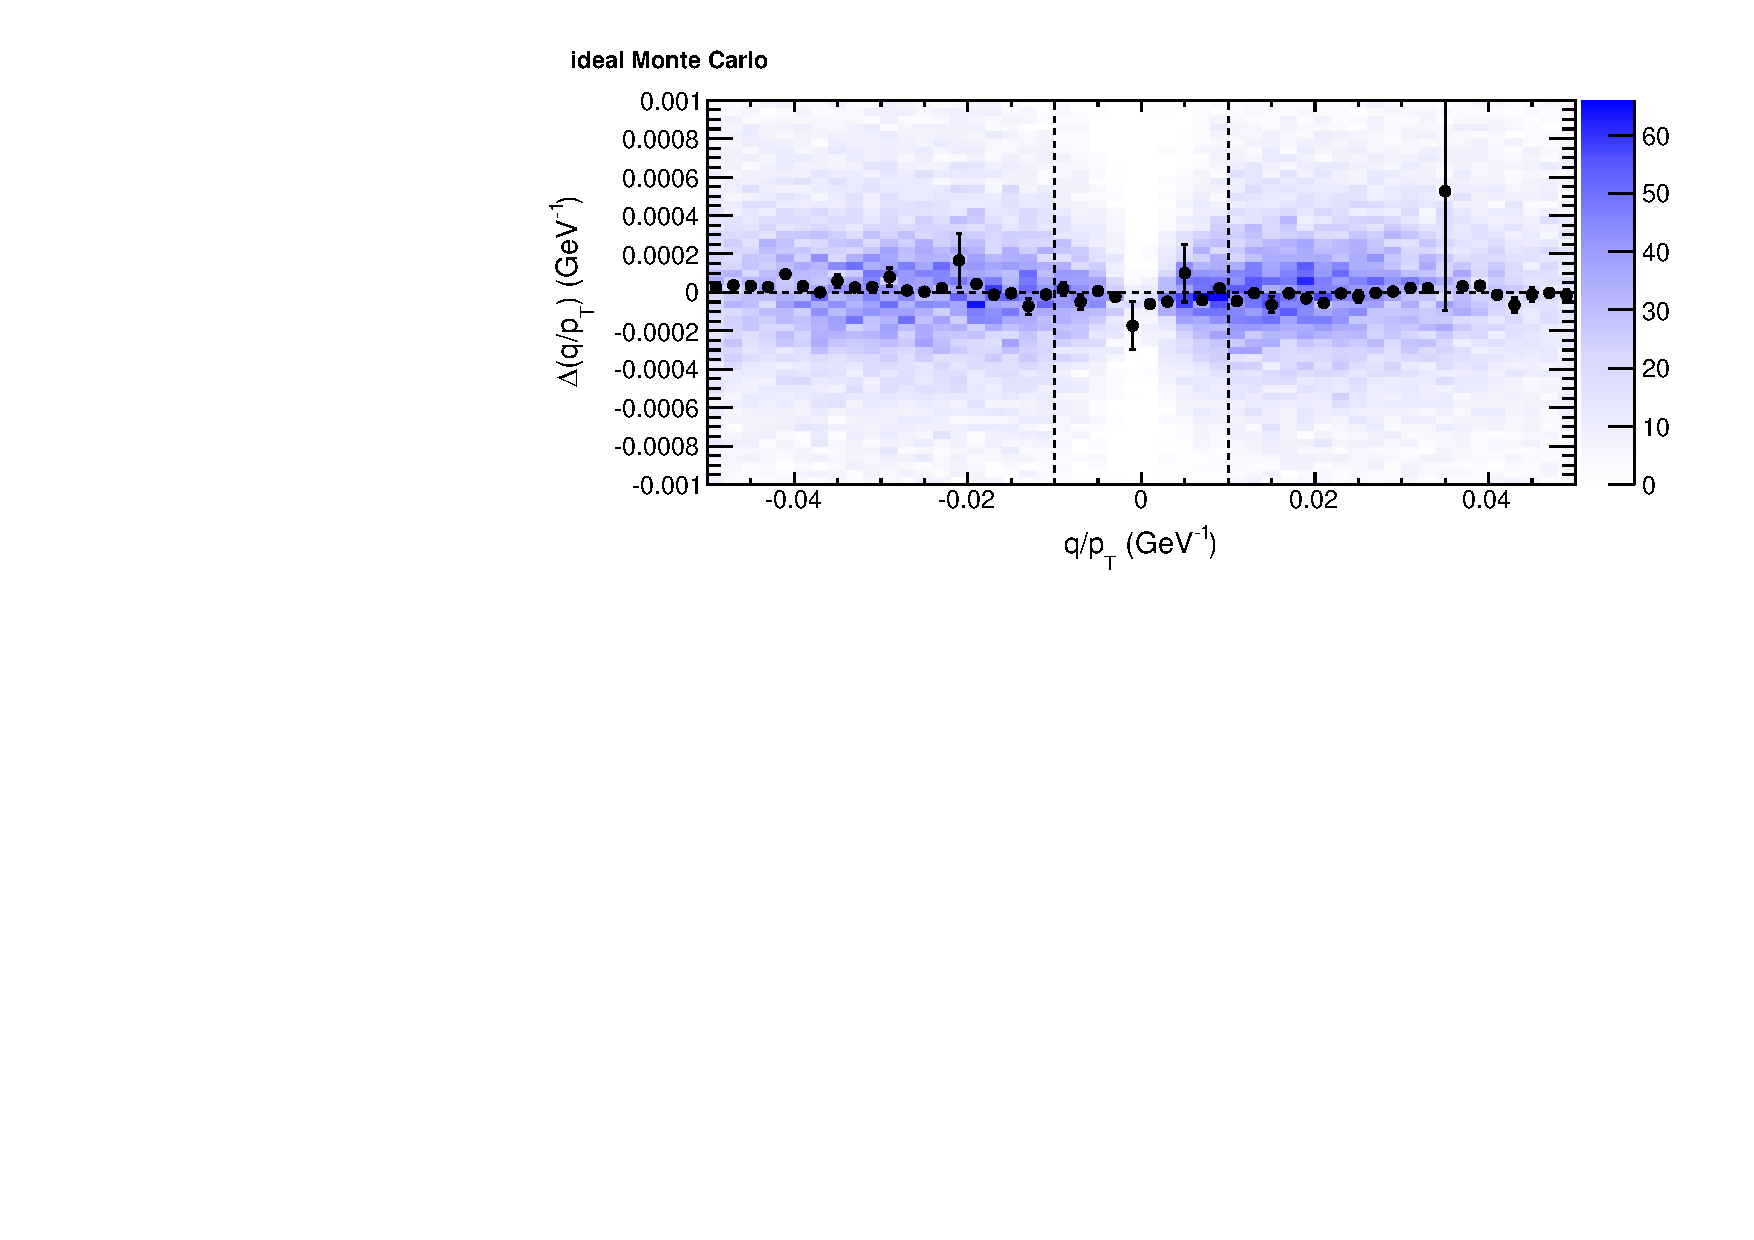
\includegraphics[width=\linewidth]{curvature_ideal.pdf}

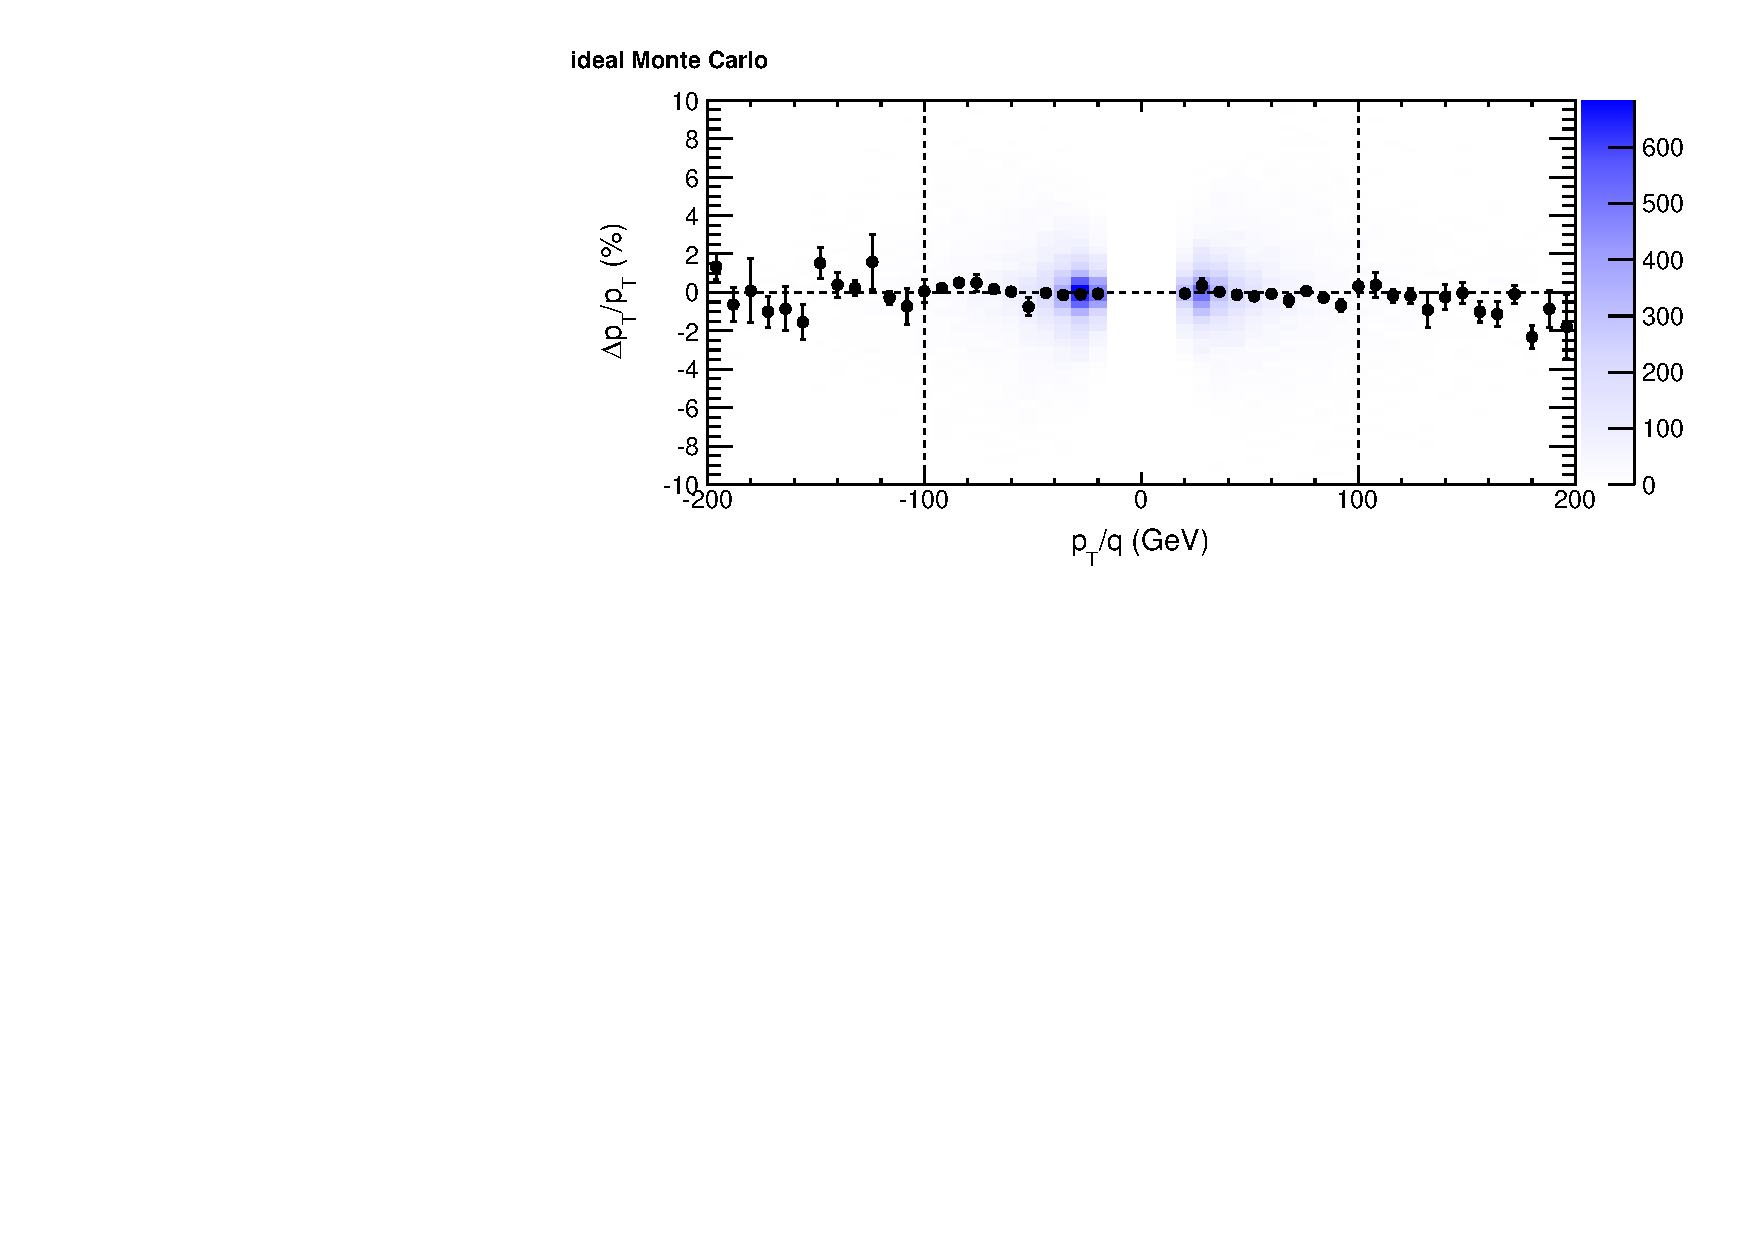
\includegraphics[width=\linewidth]{momenta_ideal.pdf}

\column{0.5\linewidth}
\begin{itemize}
\item When applied to ideal MC, everything is perfect

\item That's good (not a software problem or anything)
\end{itemize}
\end{columns}
\end{frame}

\begin{frame}
\frametitle{Straw-man global distortions (1)}

\begin{columns}
\column{0.57\linewidth}

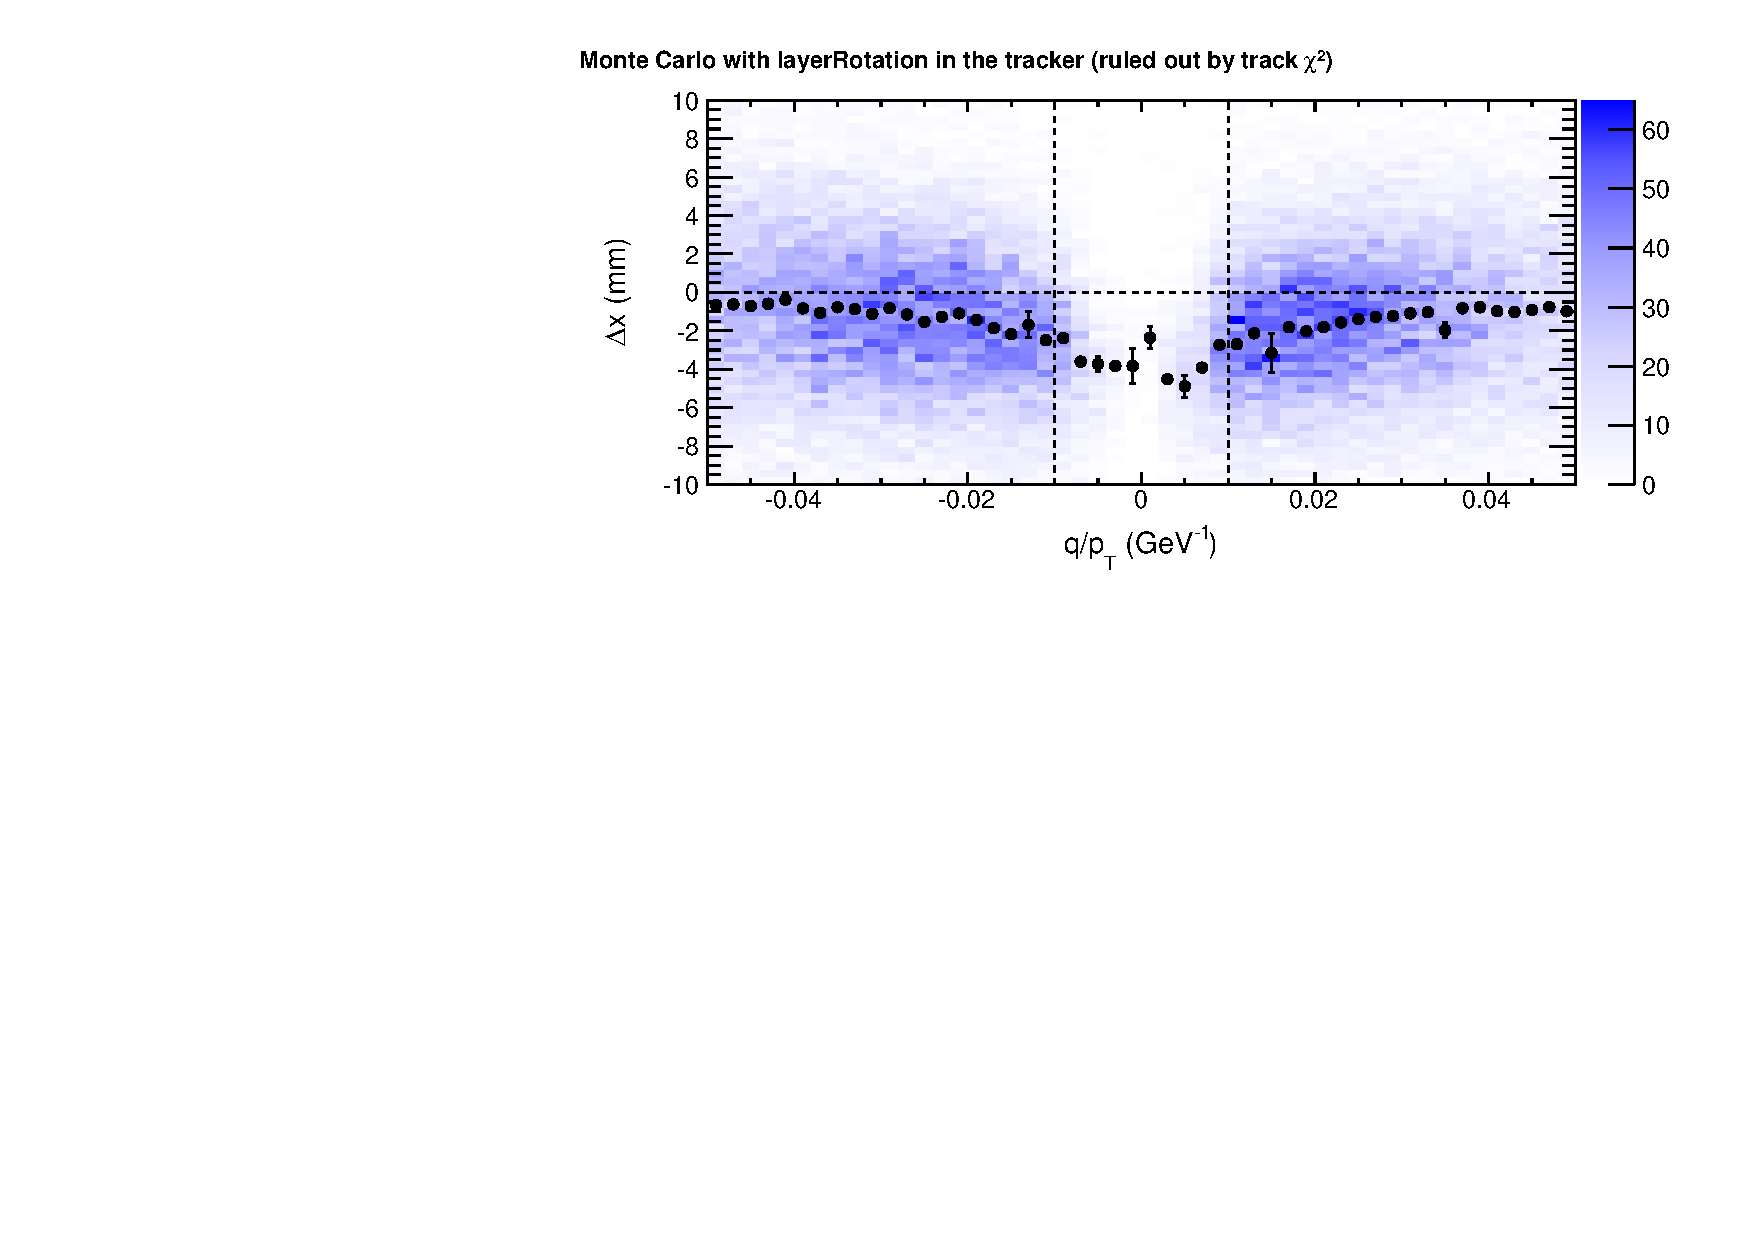
\includegraphics[width=\linewidth]{residuals_layerRotation.pdf}

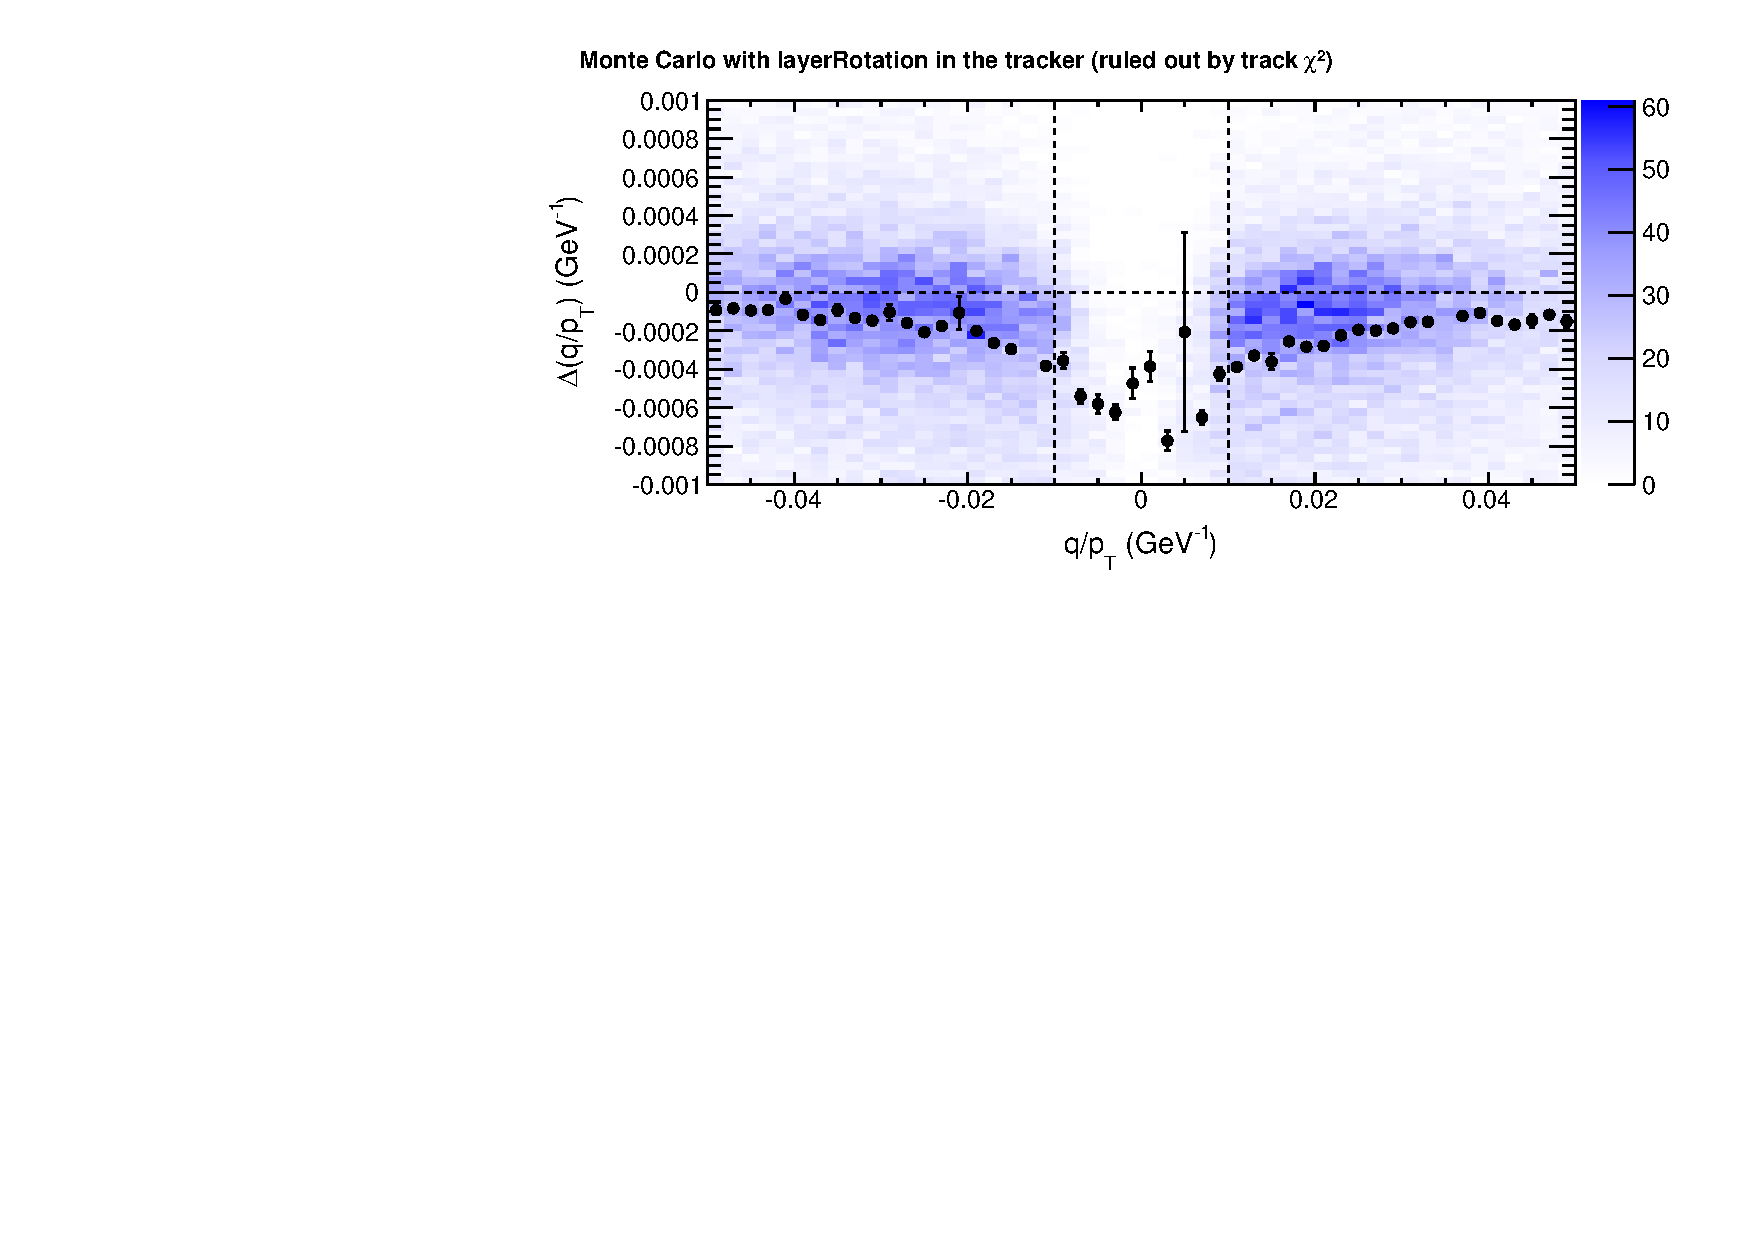
\includegraphics[width=\linewidth]{curvature_layerRotation.pdf}

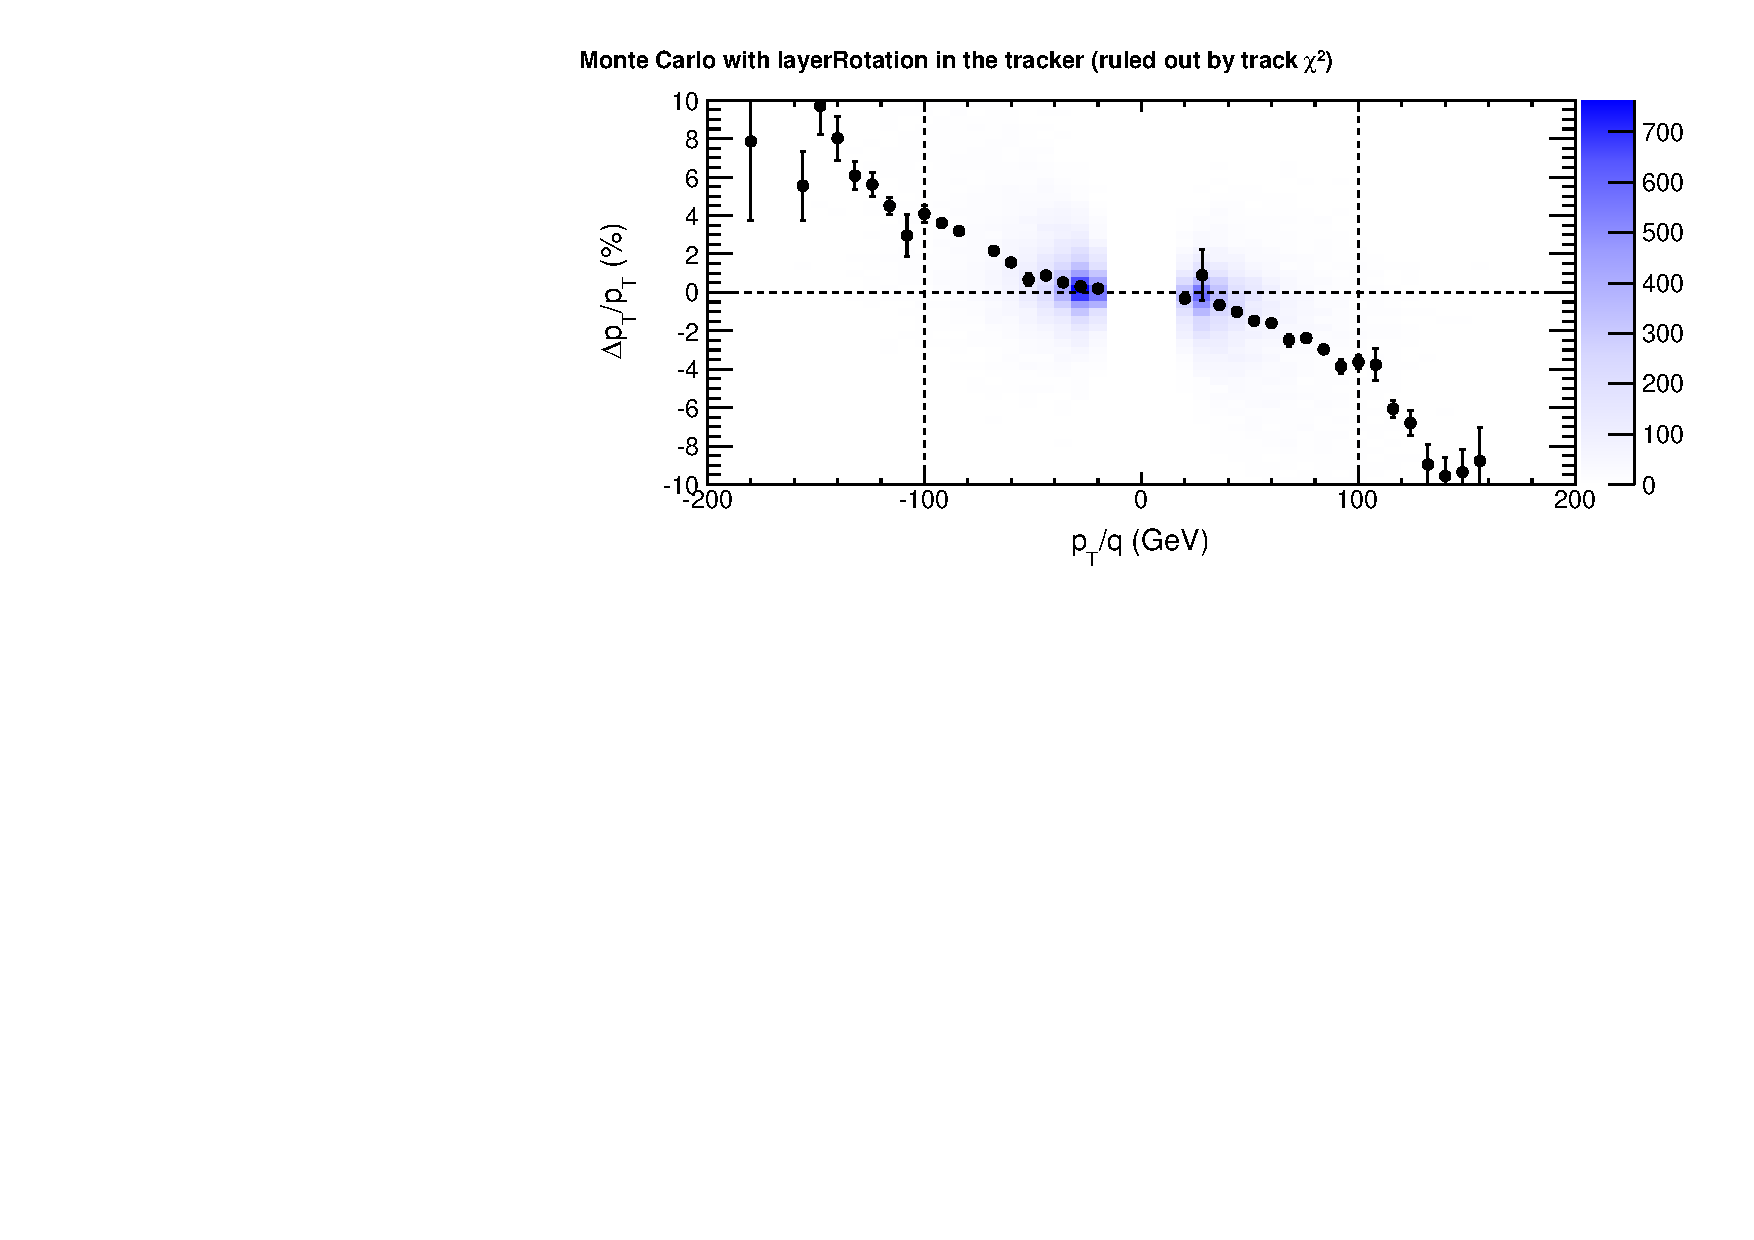
\includegraphics[width=\linewidth]{momenta_layerRotation.pdf}

\column{0.5\linewidth}
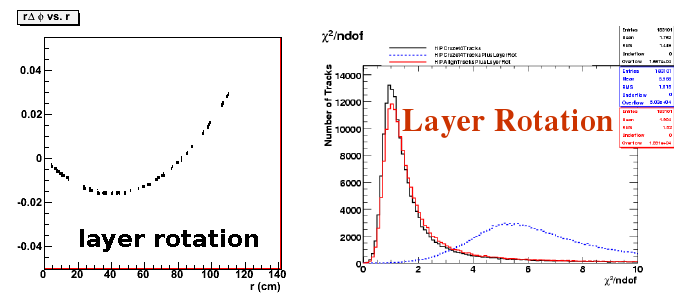
\includegraphics[width=\linewidth]{layerRotation.png}

\begin{itemize}
\item $r\phi$ rotation of tracker layers as a function of $r$

\item Tracker track $\chi^2$ is highly sensitive to this, so it has been ruled out

\item Nevertheless, it would produce a similar effect
\end{itemize}
\end{columns}
\end{frame}

\begin{frame}
\frametitle{Straw-man global distortions (2)}

\begin{columns}
\column{0.57\linewidth}

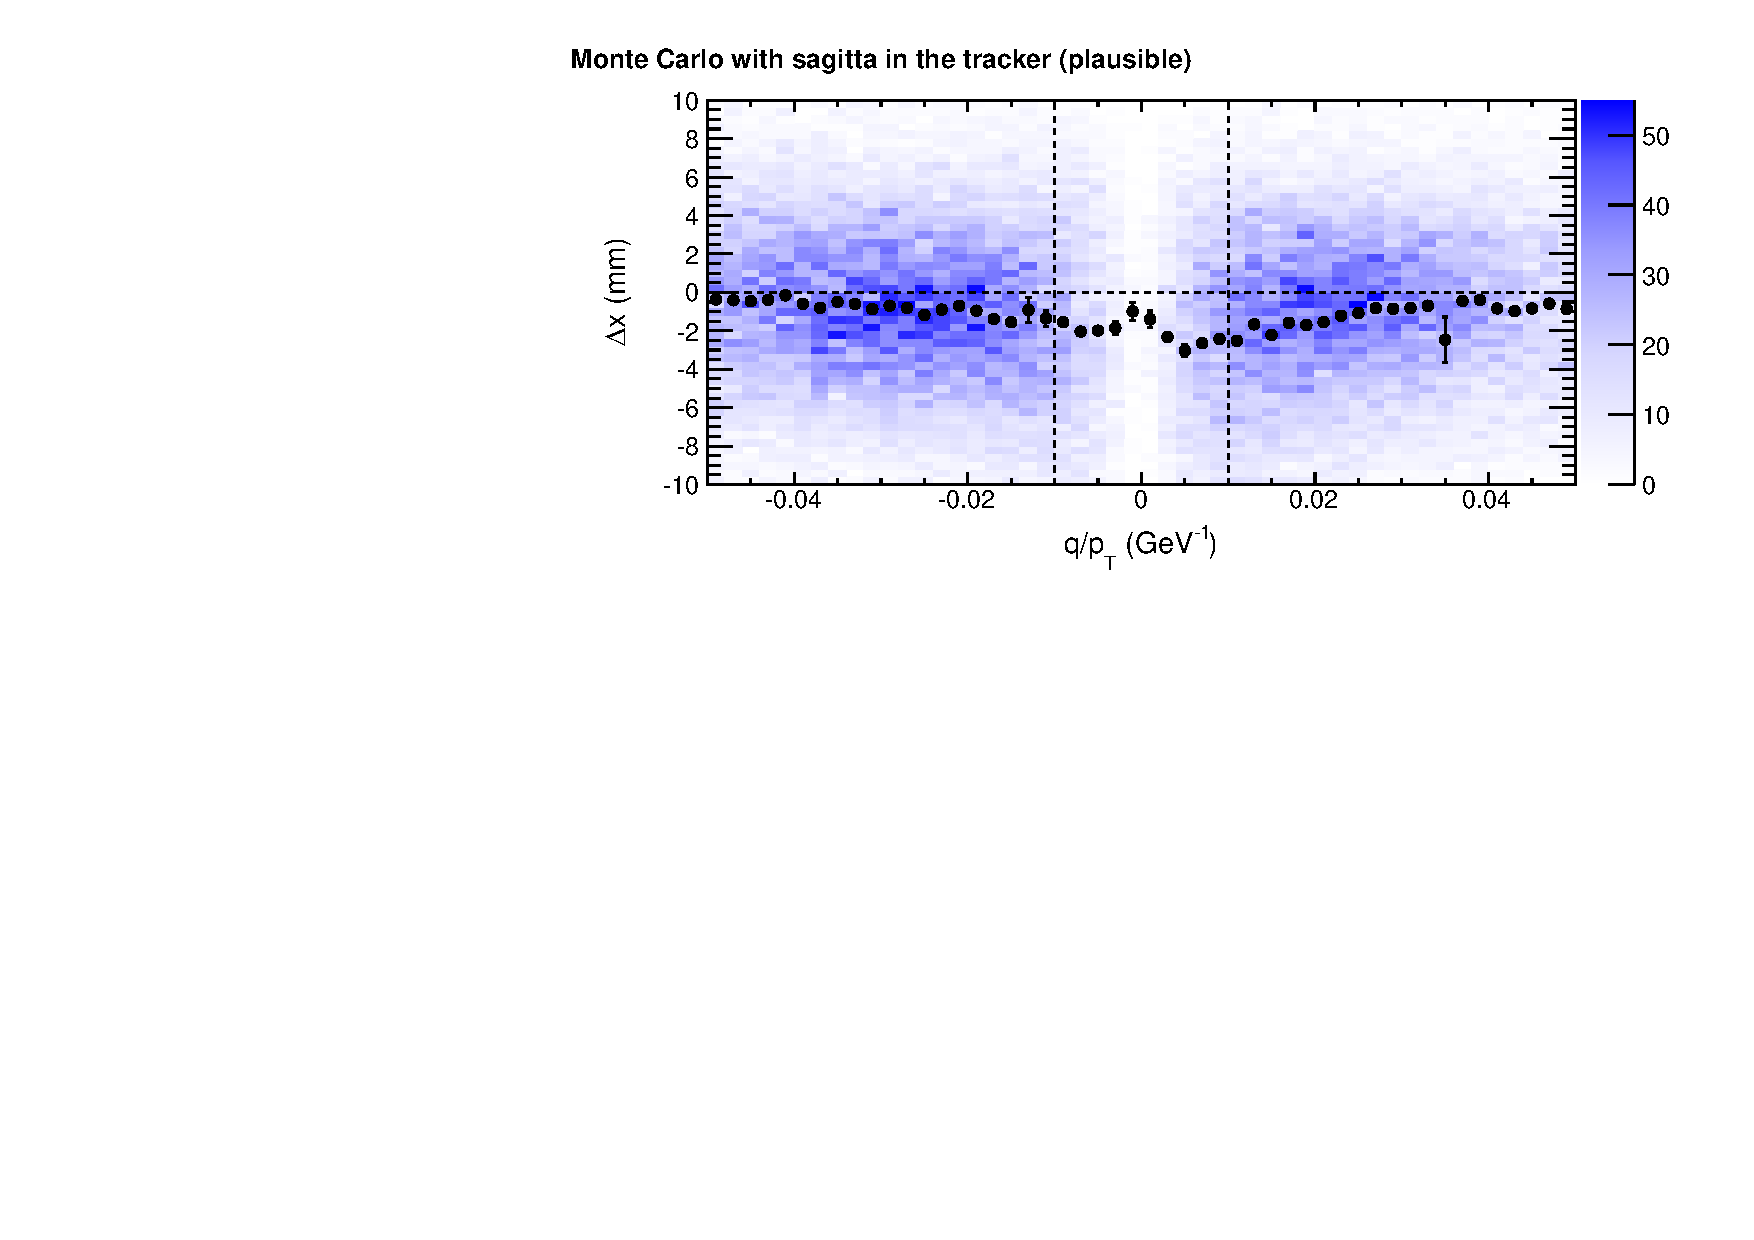
\includegraphics[width=\linewidth]{residuals_sagitta.pdf}

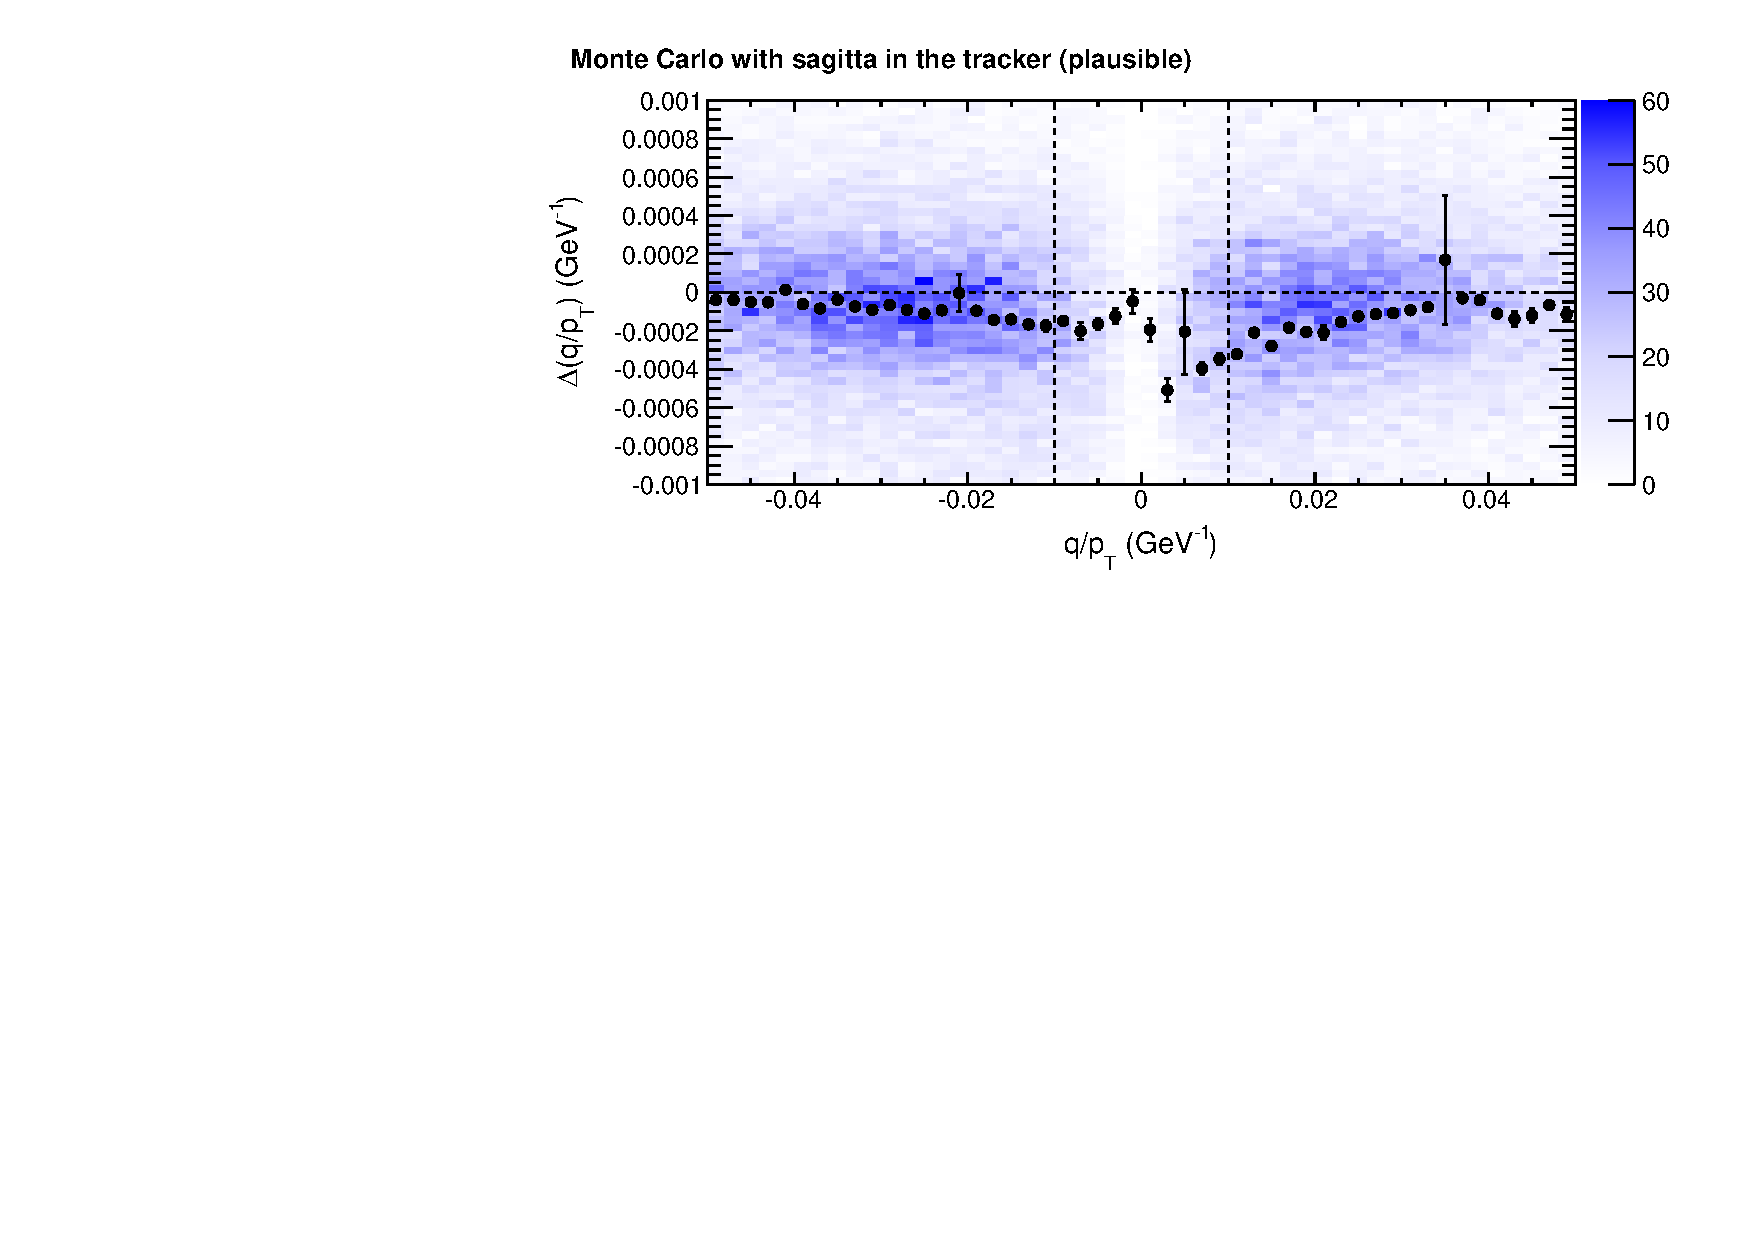
\includegraphics[width=\linewidth]{curvature_sagitta.pdf}

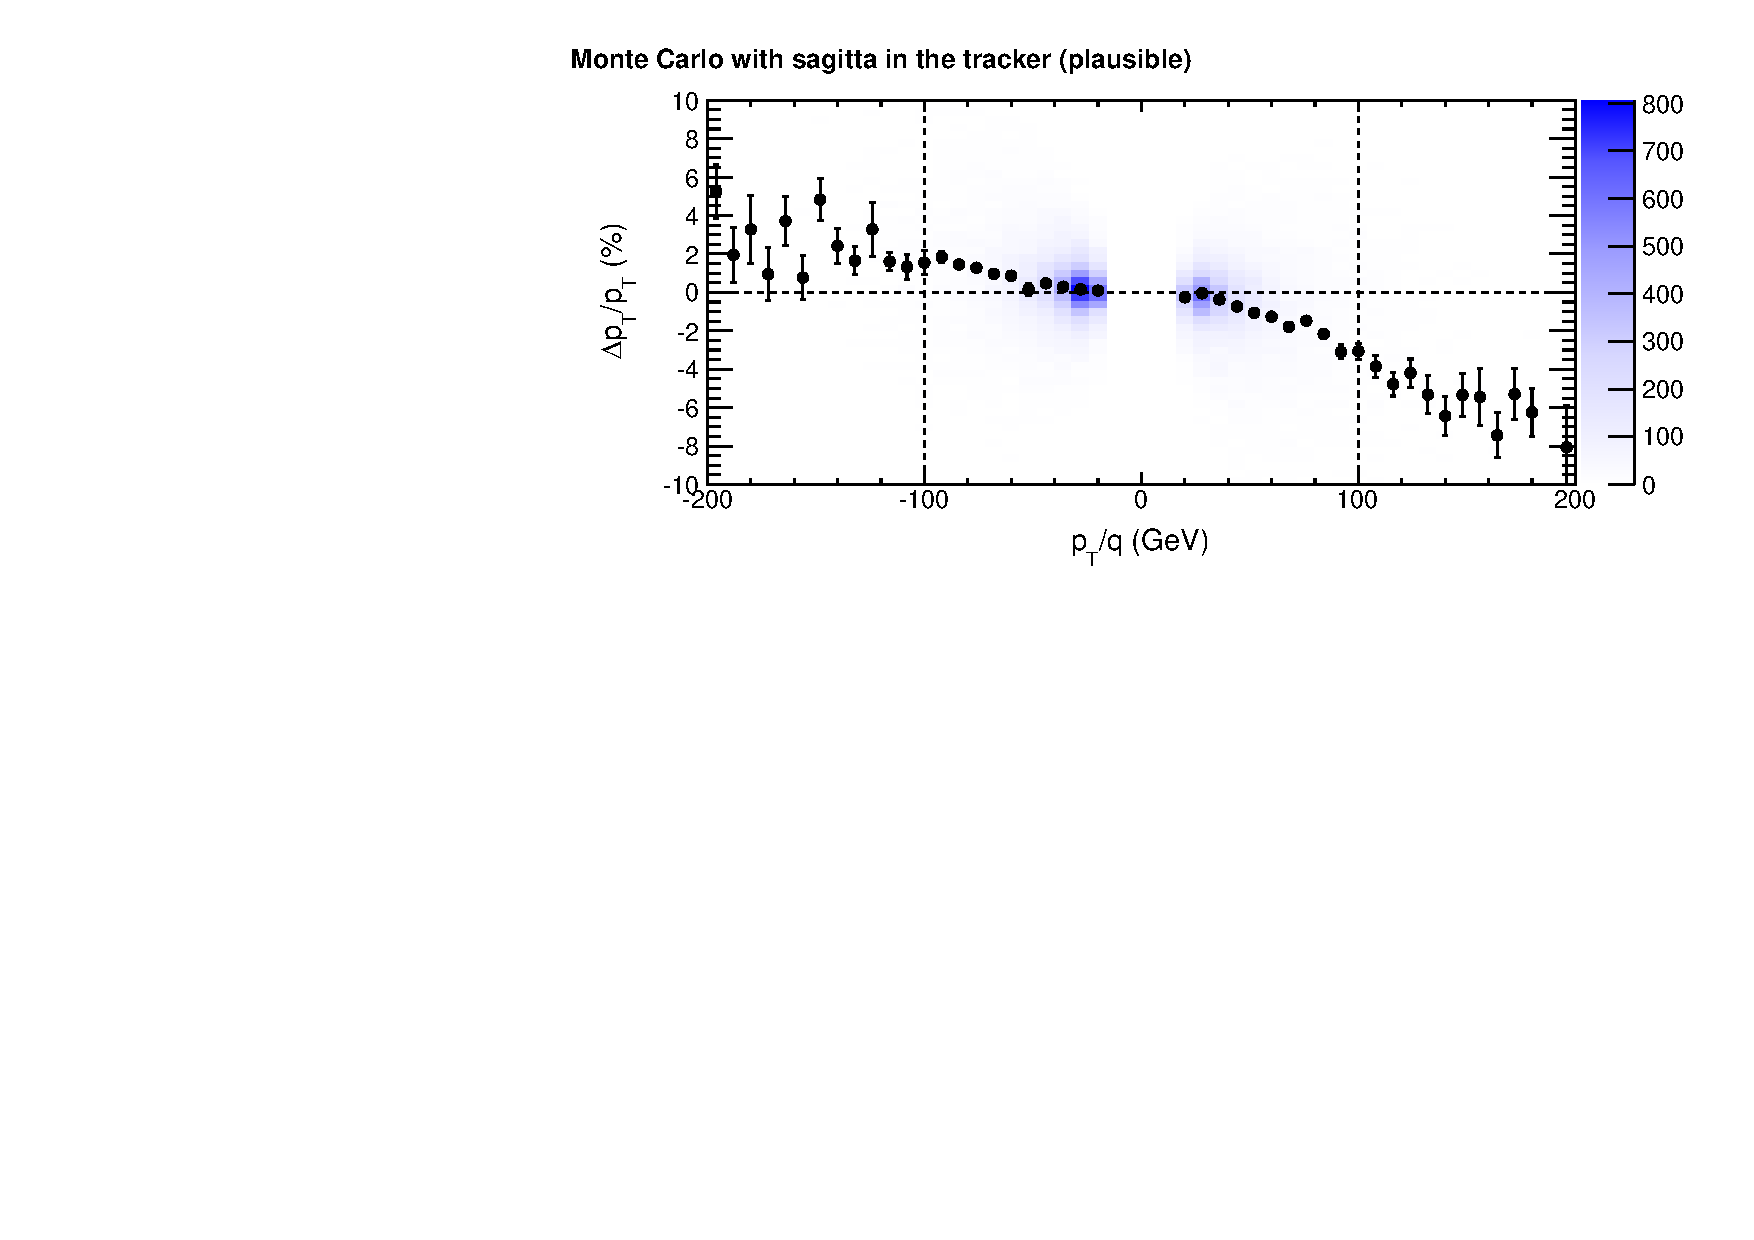
\includegraphics[width=\linewidth]{momenta_sagitta.pdf}

\column{0.5\linewidth}
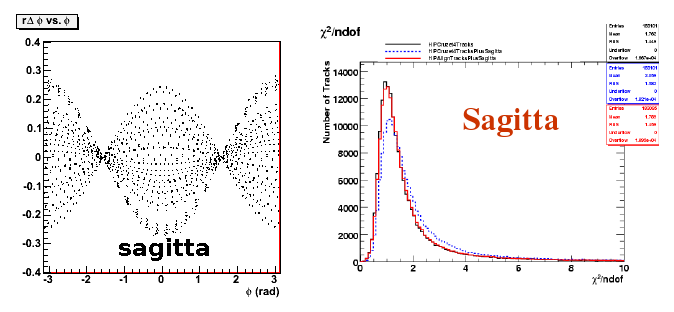
\includegraphics[width=\linewidth]{sagitta.png}

\begin{itemize}
\item $r\phi$ rotation of tracker layers as a function of $\phi$

\item Cosmic ray tracker tracks are not very sensitive to this

\item It also produces a similar effect

\item That doesn't mean that it's the only explanation
\end{itemize}
\end{columns}
\end{frame}

\begin{frame}
\frametitle{Why it's not sagitta}

\begin{itemize}
\item Plot tracker curvature error $\Delta (q/p_T)$ on the color scale (GeV$^{-1}$)
\item Horizontal axes as indicated
\end{itemize}

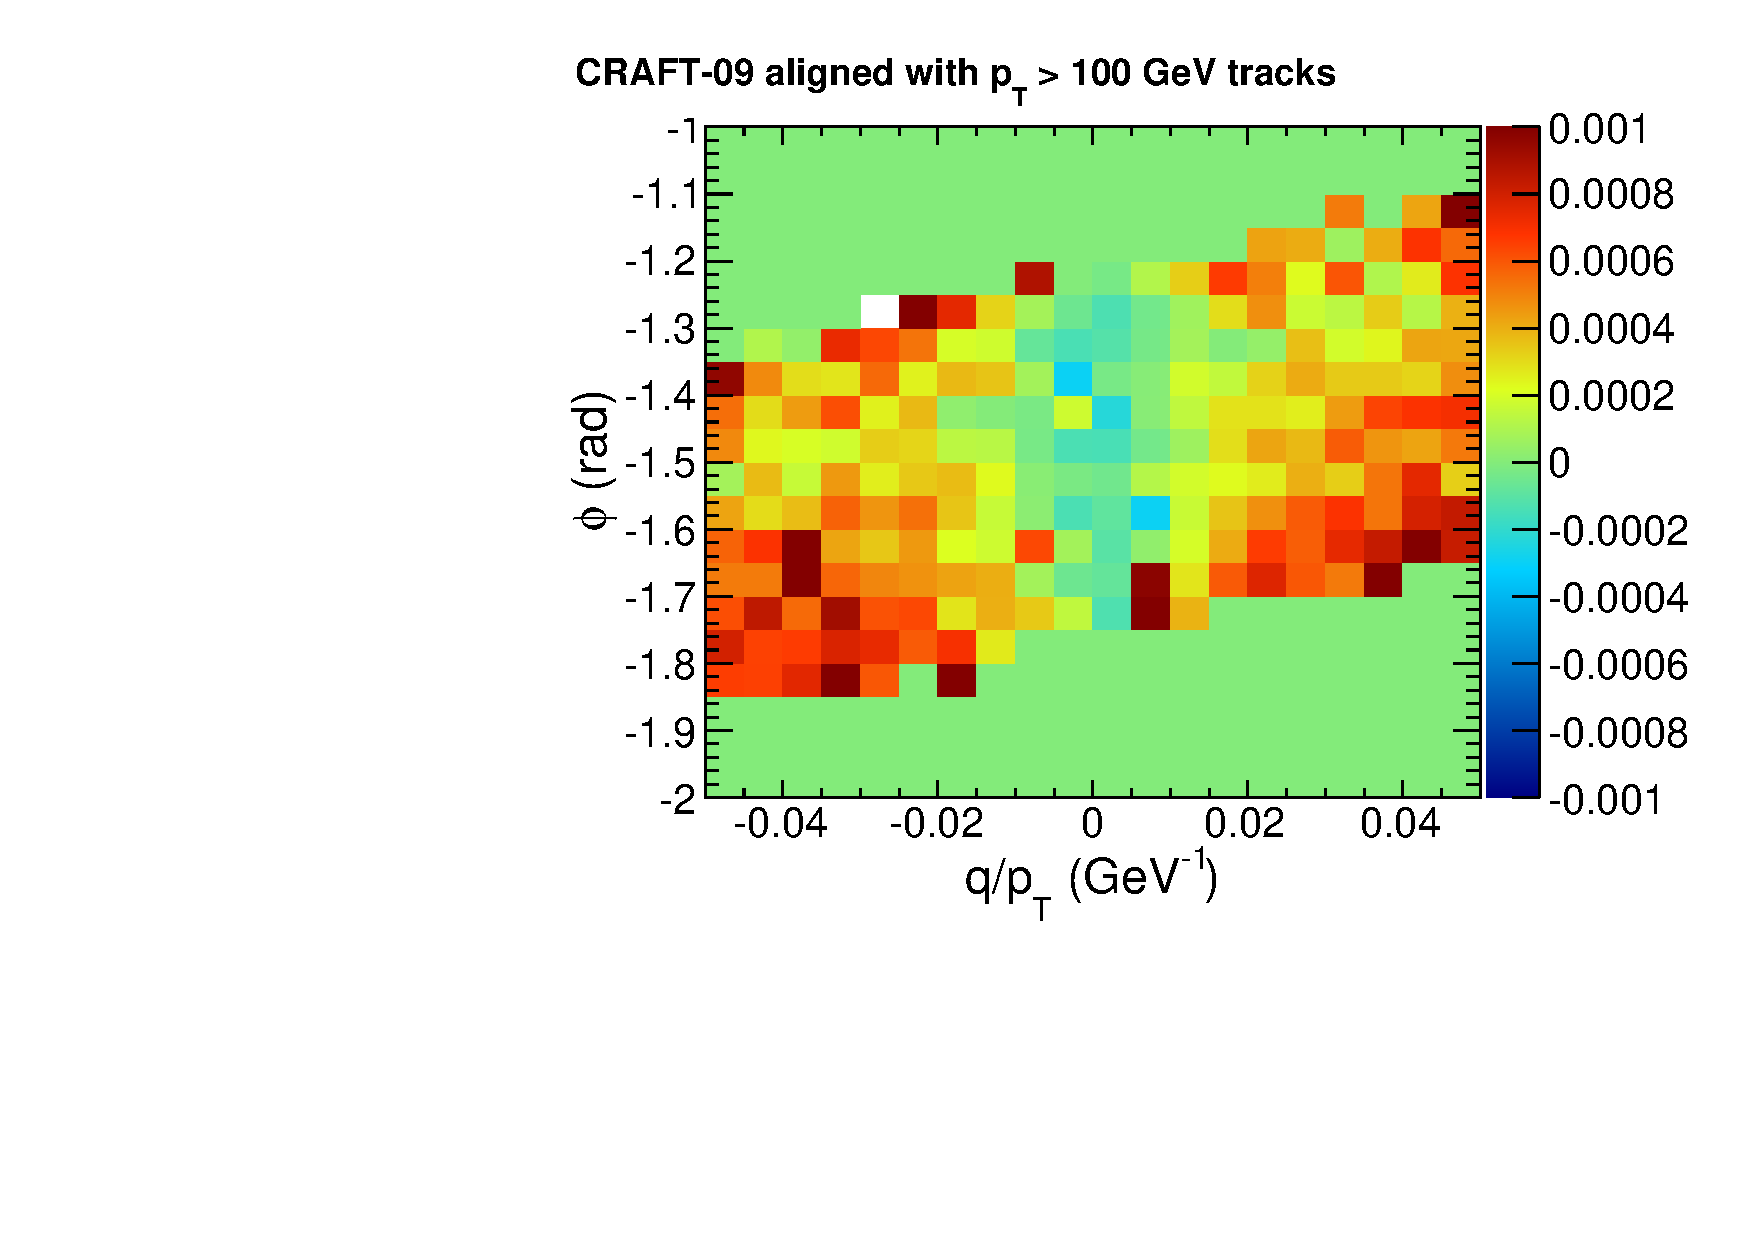
\includegraphics[width=0.5\linewidth]{2d_real.pdf}
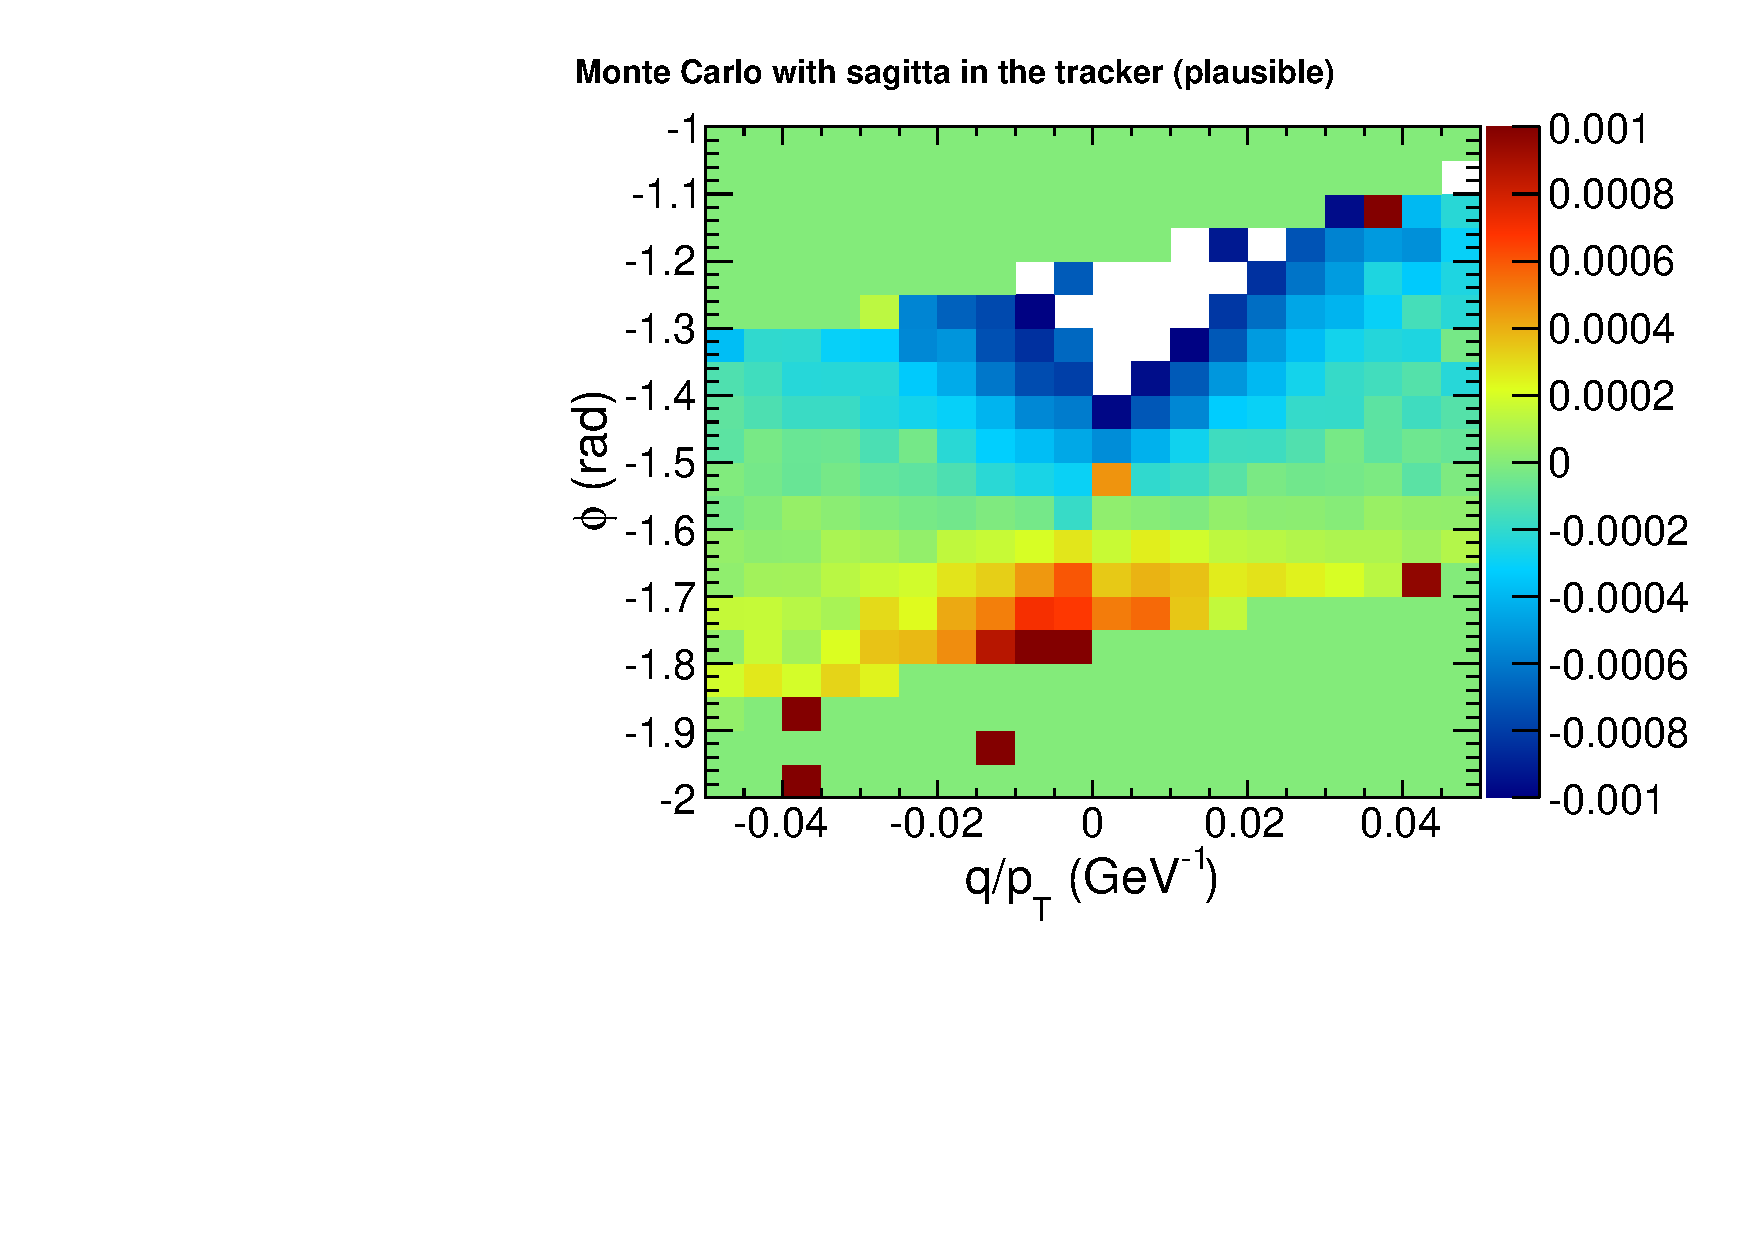
\includegraphics[width=0.5\linewidth]{2d_sagitta.pdf}

\begin{itemize}
\item Real distortion is more a function of $q/p_T$ than $\phi$
\item Sagitta error is more a function of $\phi$ than $q/p_T$
\end{itemize}

\end{frame}

%% \section*{First section}
%% \begin{frame}
%% \begin{center}
%% \Huge \textcolor{blue}{First section}
%% \end{center}
%% \end{frame}

\begin{frame}
\frametitle{Conclusions}

\begin{itemize}\setlength{\itemsep}{0.5 cm}
\item New hardware geometry is much more internally consistent

\item There are still observable discrepancies that are not due to tracker global distortions or track propagation

\item Muon residuals can be used to identify (and eventually constrain) tracker global distortions
\begin{itemize}\setlength{\itemsep}{0.25 cm}
\item turning the problem discovered in May into an asset

\item I'm trying to get people interested in using this method as a tool for tracker diagnosis: two people are possibly interested
\end{itemize}
\end{itemize}

\label{numpages}
\end{frame}

\end{document}
